%make
% !TEX TS-program = pdflatex
% !TEX encoding = UTF-8 Unicode

% This is a simple template for a LaTeX document using the "article" class.
% See "book", "report", "letter" for other types of document.

\documentclass[12pt]{article} % use larger type; default would be 10pt

\usepackage[utf8]{inputenc} % set input encoding (not needed with XeLaTeX)

%%% Examples of Article customizations
% These packages are optional, depending whether you want the features they provide.
% See the LaTeX Companion or other references for full information.

%%% PAGE DIMENSIONS
\usepackage{hyperref}
\usepackage{geometry} % to change the page dimensions
\geometry{a4paper} % or letterpaper (US) or a5paper or....
\geometry{left=2.5cm}
\geometry{right=3cm}
\geometry{top=3cm}
\geometry{bottom=3cm}
% \geometry{margin=2in} % for example, change the margins to 2 inches all round
% \geometry{landscape} % set up the page for landscape
%   read geometry.pdf for detailed page layout information

\usepackage{graphicx} % support the \includegraphics command and options

% \usepackage[parfill]{parskip} % Activate to begin paragraphs with an empty line rather than an indent

%%% PACKAGES
\usepackage{bigints}
%\usepackage[showboxes]{textpos}
\usepackage{textpos}
\usepackage{color,soul}
\usepackage{wrapfig}
\usepackage{mathtools}
\usepackage[all,cmtip]{xy}
\usepackage{mystyle}
\usepackage{xeCJK}
\usepackage{lpic}
\usepackage{etoolbox}
\usepackage{comment}
\usepackage{ulem}
\usepackage{setspace}
\usepackage{booktabs} % for much better looking tables
\usepackage{array} % for better arrays (eg matrices) in maths
\usepackage{paralist} % very flexible & customisable lists (eg. enumerate/itemize, etc.)
\usepackage{verbatim} % adds environment for commenting out blocks of text & for better verbatim
\usepackage{subfig} % make it possible to include more than one captioned figure/table in a single float
\usepackage{amssymb}
\usepackage{amsfonts}
\usepackage{amsmath}
\usepackage{xeCJK}
\usepackage{ruby}
%\renewcommand\rubysep{-5ex}
\newcommand{\kana}[2]{\ruby{#1}{#2}}
\usepackage{amssymb}
\usepackage{amsfonts}
\usepackage{amsmath,amsthm}
\usepackage{xeCJK}
\usepackage{ruby}

%CJK font
%\setCJKmainfont[AutoFakeBold=true]{MS PGothic}
\setCJKmainfont[AutoFakeBold=true]{Hiragino Mincho Pro}
% These packages are all incorporated in the memoir class to one degree or another...

%thm environments
\newtheorem{question}{質問}
\newtheorem{answer}{私の答え}
\newtheorem*{fact*}{Fact}
\newtheorem{taggedpropx}{\textbf{命題}}
\newtheorem{cor}{系}
%%\newtheorem*{proof}{証明}
\newtheorem*{lemma*}{補題}
\newtheorem{prop}{命題}

\theoremstyle{remark}
\newtheorem*{setting*}{\textbf{設定}}
\newtheorem*{goal*}{\textbf{目標}}
\newtheorem*{remark*}{\textbf{注}}
\newtheorem*{example*}{\textbf{例}}

\newcommand{\red}[1]{{\color[rgb]{0.6,0,0}#1}}
	\definecolor{Blue}{rgb}{0,0.0,1}
	\definecolor{Red}{rgb}{1,0.0,0}

\usepackage{tikz}
\usetikzlibrary{shapes,arrows,patterns}
\newcommand*\mytextcircled[1]{\tikz[baseline=(char.base)]{
	\node[shape=circle,draw,inner sep=1.8pt] (char) {\scalebox{0.8}{\kern-0.05cm #1}};}}
\newcommand{\mybigplus}{\scalebox{2.0}{$+$}}
\renewcommand{\implies}{\Rightarrow}
\newcommand{\mypgf}{{\mbox{\textbf{ガンマ関数の積}}}}
\newcommand{\Sol}{\mathcal{S}\mbox{ol}}
\newcommand{\Ind}{\mbox{\normalfont Ind}}
\newcommand{\Hom}{\mbox{\normalfont Hom}}
\newcommand{\D}{\mathcal{D}}
\newcommand{\A}{\mathcal{A}}
\newcommand{\Co}{\mathbb{C}}
\newcommand{\X}{\mathbb{X}}
\renewcommand{\setminus}{\backslash}
\newcommand{\nin}{\not\in}
\newcommand{\tmop}[1]{\ensuremath{\operatorname{#1}}}
\newcommand{\tmtextbf}[1]{{\bfseries{#1}}}
\newcommand{\tmtextit}[1]{{\itshape{#1}}}
\newcommand{\mss}{//}
\newcommand{\mbb}{\backslash\backslash}
\newcommand{\mmm}{\mid\mid}
\catcode`\<=\active \def<{
\fontencoding{T1}\selectfont\symbol{60}\fontencoding{\encodingdefault}}
\catcode`\>=\active \def>{
\fontencoding{T1}\selectfont\symbol{62}\fontencoding{\encodingdefault}}
\newcommand{\assign}{:=}
\newcommand{\comma}{{,}}
\newcommand{\um}{-}
\newcommand{\sol}{\mathcal{S}ol(\R^{p,q};\lambda,\nu)}
\newcommand{\Op}{\mbox{\normalfont Op}}
\newcommand{\Res}{\operatorname{Res}\displaylimits}
\newcommand{\OpR}{\mbox{\it R}}

\newenvironment{taggedprop}[1]
 {\renewcommand\thetaggedpropx{#1}\taggedpropx}
  {\endtaggedpropx}
%%% HEADERS & FOOTERS
\usepackage{fancyhdr} % This should be set AFTER setting up the page geometry
\pagestyle{fancy} % options: empty , plain , fancy
\renewcommand{\headrulewidth}{0pt} % customise the layout...
\lhead{}\chead{}\rhead{}
\lfoot{}\cfoot{\thepage}\rfoot{}

%%% SECTION TITLE APPEARANCE

%%% ToC (table of contents) APPEARANCE
\usepackage[nottoc,notlof,notlot]{tocbibind} % Put the bibliography in the ToC
\usepackage[titles,subfigure]{tocloft} % Alter the style of the Table of Contents
\renewcommand{\cftsecfont}{\rmfamily\mdseries\upshape}
\renewcommand{\cftsecpagefont}{\rmfamily\mdseries\upshape} % No bold!

%%%my commands
\newcommand{\mytime}[1]{\noindent #1\\}
%\newcommand{\kana}[2]{#1{ (#2)}}
\newcommand{\J}{$J(\nu)$}
\newcommand{\I}{$I(\lambda)$}
\newcommand{\doubt}[1]{\fbox{#1}}
\newcommand{\mynum}{}
\newcommand{\slowly}[1]{\dashuline{#1}}
\newcommand{\continuously}[1]{\underline{#1}}

%%% END Article customizations

%%% The "real" document content comes below...

\title{2 つのゲーゲンバウアー多項式に関連する積分公 式について}
\author{東京大学・大学院数理科学研究科、カブリ数物連携宇宙研究機構\quad 小林\quad 俊行\\
Toshiyuki Kobayashi\\
Graduate School of Mathematical Sciences,\\
the University of Tokyo,\\
Kavli Institute for the Physics and Mathematics of the Universe,\\\\
東京大学・大学院数理科学研究科\quad レオンチエフ\quad アレックス\\
Alex Leontiev\\
Graduate School of Mathematical Sciences,\\
the University of Tokyo
}
\date{} % Activate to display a given date or no date (if empty),
         % otherwise the current date is printed 

\begin{document}
\maketitle

\section{主結果}
	Gegenbauer多項式$\left\{ C_n^\lambda \right\}_{n=1}^{\infty}$は、
	$\Re(\lambda)>-\frac{1}{2}$のとき$L^2\left( [-1,1],(1-x^2)^{\lambda-\frac{1}{2}}dx \right)$の直交多項式である.
	\vspace{-0.2cm}
	\begin{example*}
		最初のいくつは
	\vspace{-0.3cm}
		\begin{eqnarray*}
	\vspace{-0.2cm}
			C_0^\lambda(x)&=&1,\\
			C_1^\lambda(x)&=&2\lambda x,\\
			C_2^\lambda(x)&=&-\lambda+2\lambda(1+\lambda)x^2,\\
			C_3^\lambda(x)&=&-2\lambda(1+\lambda)x+\frac{4}{3}\lambda(1+\lambda)(2+\lambda)x^3,\\
			C_4^\lambda(x)&=&\left(\frac{4+\lambda^3}{3}+4\lambda^2+\frac{8\lambda}{3}  \right)x^3+(-2\lambda^2-2\lambda)x.
		\end{eqnarray*}
	\end{example*}
	Gegenbauer多項式は以下のような微分方程式を満たす:
		\vspace{-0.2cm}
	\begin{equation*}
		(1-x^2)y''-(2\lambda+1)xy'+n(n+\lambda)y=0.
	\end{equation*}
	\begin{prop}\label{prop:exp-st-gg}
		$\Re\lambda,\Re\mu>-\frac{1}{2},\Re\nu>0$のとき、
		\begin{equation}
			| s + t |^{2 \nu} =b(\lambda,\mu,\nu) \sum_{\mbox{ $\begin{array}[]{c}
			\ell, m = 0 \\ \ell + m : \tmop{even}
		\end{array}$}}^{\infty} a_{\lambda,\mu,\nu}^{\ell,m} C_\ell^{\lambda} (s) C_m^{\mu} (t),
			\label{eqn:exp-st-gg}
		\end{equation}
		{
			\begin{equation*}
				\begin{array}{rcl}
	a_{\lambda,\mu,\nu}^{\ell,m}&:=&\frac{ (\lambda + \ell) (\mu + m)   }{\Gamma \left( \lambda + \nu + \frac{\ell -
	  m}{2} + 1 \right)  \Gamma \left( \mu + \nu -
	  \frac{\ell - m}{2} + 1 \right)\Gamma \left( \lambda + \mu + \nu + \frac{\ell +
	  m}{2} + 1 \right)\Gamma\left(  \nu+1-\frac{\ell+m}{2}\right)},\\[0.4cm]
	  b(\lambda,\mu,\nu)&:=&2^{-2\nu}\Gamma (\lambda + \mu + 2 \nu + 1){\Gamma (\lambda)
	  \Gamma (\mu)\Gamma \left( 2\nu +
	1 \right)}
			\end{array}
			\end{equation*}
	}
	\end{prop}
	{\bf Plan:} これの4通りの証明をあげる.
	実は、もっと一般的な主張が成り立つ:
	\begin{prop}\label{prop:exp-stz-gg}
		  \label{thm:4}$\tmop{Re} \lambda, \tmop{Re} \mu > - \frac{1}{2}$,
		    $\tmop{Re} \nu > 0$ と $-1 \leqslant z \leqslant 1$ のとき、
		      \begin{eqnarray}
			      & | s + t z |^{2 \nu}  = \sum_{\scalebox{0.6}{
				      $\begin{array}[]{c}
						  \ell,m=0\\\ell+ m\mbox{ :even}
					  \end{array}
				  $}}^{\infty} a_{\ell, m}
					          (z) C_\ell^{\lambda} (s) C_m^{\mu} (t), &  \nonumber\\
						      & a_{\ell, m} (z) = \frac{\Gamma \left( \nu + \frac{1}{2} \right) \Gamma
						      (\lambda) \Gamma (\mu) (\lambda + l) z^m }{(1 + \nu)_{- \frac{\ell + m}{2}} \sqrt{\pi} \Gamma
										      (\mu + m) \Gamma \left( \lambda + \nu + \frac{\ell - m}{2} + 1 \right)}&\nonumber
										      \\&\times{}_2 F_1 \left( \begin{array}{c}
								        \frac{\ell + m}{2} - \nu, \frac{m - \ell}{2} - \nu - \lambda\\
									      \mu + m + 1
									          \end{array} ; z^2 \right). & 
										          \nonumber
											    \end{eqnarray}
    \end{prop}
    命題\ref{prop:exp-st-gg}は命題\ref{prop:exp-stz-gg}において$z=1$を代入したときの結果である.
	命題\ref{prop:exp-st-gg}は次の
	積分公式と同値である.
	\begin{taggedprop}{$\;\mathbf{1'}$}
		\label{prop:int-st-gg}
		\begin{equation*}
			\int_{- 1}^1 \int_{- 1}^1 | s - t |^{2 \nu} (1 - s^2)^{\lambda - \frac{1}{2}}
			(1 - t^2)^{\mu - \frac{1}{2}} C_\ell^{\lambda} (s) C_m^{\mu} (t) d s d t
		\end{equation*}
		{
		\begin{equation}
			=\frac{(- \nu)_{\frac{\ell + m}{2}} (- 1)^{\frac{\ell - m}{2}} \pi^{\frac{1}{2}} (2
			\lambda)_\ell (2 \mu)_m \Gamma \left( \lambda + \frac{1}{2} \right) \Gamma \left(
			\mu + \frac{1}{2} \right) \Gamma \left( \nu + \frac{1}{2} \right) \Gamma
		(\lambda + \mu + 2 \nu + 1)}{\ell!m! \Gamma \left( \lambda + \nu + \frac{\ell -
		m}{2} + 1 \right) \Gamma \left( \mu + \nu - \frac{\ell - m}{2} + 1 \right) \Gamma
		\left( \lambda + \mu + \nu + \frac{\ell + m}{2} + 1 \right)}
			\label{eqn:int-st-gg}
			\tag{1$'$}
		\end{equation}
		}
	\end{taggedprop}
	ここでポッホハマー記号$(x)_n$は以下のように定義される:\begin{equation*}
		(x)_n:=\frac{\Gamma(x+n)}{\Gamma(x)}=x(x+1)\cdots(x+n-1).
	\end{equation*}
\section{主結果の様々な特殊化}
エルミート多項式$\left\{ H_n \right\}_{n=1}^\infty$は、
	$L^2\left( \mathbb{R},e^{-\frac{x^2}{2}}dx \right)$の直交多項式である.
	\begin{example*}
		最初のいくつは
	\vspace{-0.3cm}
		\begin{eqnarray*}
		H_0(x)&=& 1,\\
		H_1(x)&=& 2x,\\
		H_2(x)&=& 
		4x^2-2,\\
		H_3(x)&=& 8x^3-12x,\\
		H_4(x)&=& 16x^4-48x^2+12.\\
		\end{eqnarray*}
	\end{example*}
	エルミート多項式はGegenbauer多項式の極限として再現できる:
	%%\vspace{-0.3cm}
	\begin{equation*}
			H_n (x) = n! \lim_{\lambda \rightarrow \infty} \lambda^{- \frac{n}{2}}
			C_n^{\lambda} \left( \frac{x}{\sqrt{\lambda}} \right).
	\end{equation*}
	命題 \ref{prop:int-st-gg}で $\lambda,\mu\to\infty$ 
	という極限をとれば(ただし、$\mu/\lambda=w\in\mathbb{R}$を一定にして極限をとる)、Gegenbauer多項式に関する積分公式(命題\ref{prop:int-st-gg})から
	エルミート多項式に関する積分公式を得る.
	\begin{cor}\label{cor:int-xzy-hh}
		$\nu\in\mathbb{C}$と$w\in\R$に対して、以下の公式が成り立つ:
		\begin{equation*}
			\begin{array}[]{c}
			\int_{- \infty}^{\infty} \int_{- \infty}^{\infty} | x - w y |^{2 \nu} e^{-
			x^2 - y^2} H_\ell (x) H_m (y) d x d y \\= (- \nu)_{\frac{\ell + m}{2}} (- 1)^{\frac{\ell
			- m}{2}} 2^{\ell + m} \pi^{\frac{1}{2}} \Gamma \left( \frac{1}{2} + \nu \right)
			(w^2 + 1)^{\nu - \frac{\ell + m}{2}} w^m .
			\end{array}
		\end{equation*}
	\end{cor}
		\begin{fact*}[Mehta積分]
			{
		\begin{equation*}
			\begin{array}[]{c}
			{(2\pi)^{-\frac{k}{2}}}\displaystyle\int_{\mathbb{R}^k}\prod_{1\le i<j\le k}\myabs{t_i-t_j}^{2\gamma}\exp\left( -\myabs{\mathbf{t}}^2/2 \right)d\mathbf{t}\\
			=\displaystyle\prod_{j=1}^k\frac{\Gamma\left( 
			1+j\gamma\right)}{\Gamma(1+\gamma)}.
			\end{array}
		\end{equation*}
	}
		\end{fact*}
		\centerline{
		\xymatrix{
			\mbox{系1}\ar@{=>}[rd]_{\begin{array}[]{c}
			w=-1,\\\ell=m=0
		\end{array}}&&\mbox{Fact}\ar@{=>}[ld]^{\begin{array}[]{c}
		k=2
	\end{array}}\\
			&&
		}}
		\begin{equation*}
			\int_{-\infty}^\infty\int_{-\infty}^\infty\myabs{x-y}^{2\nu}e^{-x^2-y^2}dxdy=\mypgf
		\end{equation*}
			\begin{figure}[h]
				\centering
				\begin{tikzpicture}
				\draw[color=black] (0.0,0.0) rectangle (2.0,-0.5);
\node at (1.0,-0.25) {\color{black}{\scriptsize Warnaar'10: \color{blue}{4}}};
\draw[color=red] (2.1,0.0) rectangle (4.3,-0.5);
\node at (3.2,-0.25) {\color{red}{\scriptsize 命題 2: \color{blue}{4}}};
\draw[color=black] (5.7,0.0) rectangle (8.9,-0.5);
\node at (7.300000000000001,-0.25) {\color{black}{\scriptsize Tarasov-Varchenko'03: \color{blue}{3}}};
\draw[color=black] (9.1,0.0) rectangle (12.1,-0.5);
\node at (10.6,-0.25) {\color{black}{\scriptsize Dotsenko-Fateev'85: \color{blue}{4}}};
\draw[color=red] (2.1,-2.0) rectangle (4.3,-2.5);
\node at (3.2,-2.25) {\color{red}{\scriptsize 命題 $1'$: \color{blue}{3}}};
\draw[color=black] (5.0,-2.0) rectangle (6.7,-2.5);
\node at (5.85,-2.25) {\color{black}{\scriptsize Selberg'44: \color{blue}{3}}};
\filldraw[color=red,pattern color=red,pattern=north east lines] (3.2,-4.0) circle(0.3);
\node at (3.85,-4.0) {\color{blue}{3}};
\fill[color=black] (1.5,-6.0) circle(0.1);
\node at (1.95,-6.0) {\color{blue}{2}};
\fill[color=black] (3.2,-6.0) circle(0.1);
\node at (3.6500000000000004,-6.0) {\color{blue}{2}};
\fill[color=black] (5.85,-6.0) circle(0.1);%TV
\node at (6.3,-6.0) {\color{blue}{2}};
\fill[color=black] (8.9,-6.0) circle(0.1);%DF
\node at (9.35,-6.0) {\color{blue}{2}};

\draw[->,>=angle 90,color=black] (2.0,-0.5) -- node {} (5.0,-2.0) ;
\draw[->,>=angle 90,color=red] (3.2,-0.5) -- node {} (3.2,-2.0) ;
\draw[->,>=angle 90,color=black] (6.18,-0.5) -- node {} (5.85,-2.0) ;
\draw[->,>=angle 90,color=black] (9.1,-0.5) -- node {} (6.615,-2.0) ;
\draw[->,>=angle 90,color=red] (3.2,-2.5) -- node {\color{black}{\scriptsize $\kern1.5cm\ell=m=0$}} (3.2000000000000006,-3.7) ;
\draw[->,>=angle 90,color=black] (1.0,-0.5) -- node {} (1.490946425395748,-5.90041067935323) ;
\draw[->,>=angle 90,color=black] (3.0057054739713385,-4.2285817953278375) -- node {} (1.5573628100792203,-5.93251434108327) ;
\draw[->,>=angle 90,color=black] (3.2,-4.3) -- node {} (3.2,-5.914999999999999) ;
\draw[->,>=angle 90,color=black] (3.4394567450999696,-4.180722071773562) -- node {} (5.777393604812446,-5.9452027206131675) ;
\draw[->,>=angle 90,color=black] (3.4830799946398643,-4.099326313908724) -- node {} (8.810326217188193,-5.968535514802874) ;
\draw[->,>=angle 90,color=black] (5.34,-2.5) -- node {} (3.252164719493017,-5.914683869988056) ;
\draw[->,>=angle 90,color=black] (10.3,-0.5) -- node {}  (8.92466,-5.90309);%DF->DF'
\draw[->,>=angle 90,color=black] (7.62,-0.5) -- node {} (5.88,-5.9048) ;%TV->TV'

				\end{tikzpicture}
				\caption{
					ここで{\color{blue}{青い数字}}は連続パラメータの個数を表す.
				}
%%				\label{fig:}
			\end{figure}
    			\setulcolor{Blue}
		\normalfont
		\begin{fact*}[{\cite{Selberg:411367}}]
	 \begin{equation*}
		\begin{array}[]{c}
		\displaystyle\int_{t \in [0, 1]^k} \displaystyle\prod\displaylimits_{i=1}^k t_i^{\alpha-1}(1-t_i)^{\beta-1} 
		\kern-0.1cm\displaystyle\prod\displaylimits_{1\le i<j\le k}\myabs{t_i-t_j}^{2\gamma} d
				t\\=\mypgf,\\
				\tmop{Re} (\alpha), \tmop{Re} (\beta) > 0, | \gamma | \ll 1.
		\end{array}
			\end{equation*}
		\end{fact*}
			\begin{fact*}[\ul{Warnaar'10} (1.4)]
				{
		\begin{equation*}
%%			\kern-2.15cm
			\begin{array}{c}
				\displaystyle\int\displaylimits_{(t,s)\in C_{\beta_1,\gamma}^{k_1,k_2}}
				\displaystyle\prod\displaylimits_{i=1}^{k_1}t_i^{\alpha_1-1}(1-t_i)^{\beta_1-1}\\
				\times\displaystyle\prod\displaylimits_{j=1}^{k_2}s_j^{\alpha_2-1}(1-s_j)^{\beta_2-1}
				\displaystyle\prod_{1\le i<j\le k_1}\myabs{t_i-t_j}^{2\gamma}\\
				\times\displaystyle\prod_{1\le i<j\le k_2}\myabs{s_i-s_j}^{2\gamma}
				\displaystyle\prod_{i,j=1}^{k_1,k_2}\myabs{t_i-s_j}^{-\gamma}dsdt
%%				\displaystyle\bigintssss_{ \mbox{$\kern1.9cm (t,s)\kern-0.1cm\in\kern-0.1cm C_{\beta_1, \gamma}^{k_1, k_2} [0, 1]$}} \kern-1.95cm\textstyle\prod^{\alpha_1 - 1,
%%				\beta_1 - 1}\kern-0.05cm (t) \kern-0.09cm\textstyle\prod^{\alpha_2 - 1, \beta_2 - 1}\kern-0.05cm (s)
%%%%					    \\ \times
%%					    \Delta^{2 \gamma}\kern-0.05cm(t)
%%					      \Delta^{2 \gamma}\kern-0.05cm (s) \Delta^{- \gamma}\kern-0.05cm (t, s)\\
				      \end{array}\end{equation*}
%%			\vspace{-0.5cm}
		\begin{equation*}
			\begin{array}{c}
					        = \mypgf,\\
%%					  \textstyle\prod^{\alpha_1 - 1,
%%					  \beta_1 - 1} (t):=\displaystyle\prod_{i=1}^{k_1}t_i^{\alpha_1-1}(1-t_i)^{\beta_1-1},\\
%%					  \Delta^{2\gamma}(t):=\displaystyle\prod_{1\le i<j\le k_1 }\kern-0.2cm\myabs{t_i}^{2\gamma}, \Delta^\gamma(t,s):=\displaystyle\prod\displaylimits_{i,j=1}^{k_1,k_2}
%%					  \myabs{t_i-s_j}^{\gamma}\kern-0.1cm,\\
%%					  \\
					  \mbox{ここで  }C^{k_1,k_2}_{\beta_1,\gamma}\mbox{: ある特異チェイン, }
					  \beta_1 + \beta_2 = \gamma + 1,\\
					    \tmop{Re} (\alpha_i), \tmop{Re} (\beta_i) > 0,  \myabs{\gamma} \ll 1 ,\\ \quad 1
						\le \forall i \le \displaystyle\min_i \{ k_i \} : \beta_1 + (i - k_2 - 1)
						  \gamma \nin \mathbb{Z}.
			\end{array}
			\end{equation*}
				}
			\end{fact*}
		\begin{fact*}[{\ul{Tarasov-Varchenko'03}}]
			{
		\begin{equation*}
%%			\kern-1.45cm
			\begin{array}{c}
				\displaystyle\int_{(t,s)\in C_\gamma^{k_1,k_2}}
				\displaystyle\prod\displaylimits_{i=1}^{k_1}t_i^{\alpha-1}(1-t_i)^{\beta_1-1}\\
				\times\displaystyle\prod\displaylimits_{j=1}^{k_2}(1-s_j)^{\beta_2-1}
				\displaystyle\prod_{1\le i<j\le k_1}\myabs{t_i-t_j}^{2\gamma}\\
				\times\displaystyle\prod_{1\le i<j\le k_2}\myabs{s_i-s_j}^{2\gamma}
				\displaystyle\prod_{i,j=1}^{k_1,k_2}\myabs{t_i-s_j}^{-\gamma}dsdt
%%				\displaystyle\bigintssss_{ \mbox{$\kern1.4cm (t,s)\kern-0.1cm\in\kern-0.1cm C_{\gamma}^{k_1, k_2} [0, 1]$}} \kern-1.65cm\textstyle\prod^{\alpha - 1,
%%				\beta_1 - 1}\kern-0.05cm (t) \kern-0.09cm\textstyle\prod^{0, \beta_2 - 1}\kern-0.05cm (s)
%%%%					    \\ \times
%%					    \Delta^{2 \gamma}\kern-0.05cm(t)
%%					      \Delta^{2 \gamma}\kern-0.05cm (s) \Delta^{- \gamma}\kern-0.05cm (t, s)\\
				      \end{array}\end{equation*}
%%			\vspace{-0.5cm}
%%			\kern-0.29cm
			      \begin{equation*}
			\begin{array}{c}
					        = \mypgf\\
					  \mbox{ここで、  }	C^{k_1,k_2}_{\gamma}\mbox{: ある特異チェイン}.\\
%%					  \textstyle\prod^{\alpha - 1,
%%					  \beta_1 - 1} (t):=\displaystyle\prod_{i=1}^{k_1}t_i^{\alpha-1}(1-t_i)^{\beta_1-1},\\
%%					  \Delta^{2\gamma}(t):=\displaystyle\prod_{1\le i<j\le k_1 }\kern-0.2cm\myabs{t_i}^{2\gamma}, \Delta^\gamma(t,s):=\displaystyle\prod\displaylimits_{i,j=1}^{k_1,k_2}
%%					  \myabs{t_i-s_j}^{\gamma}\kern-0.1cm.\\
%%					  \\
%%					\tmop{Re} (\alpha_i), \tmop{Re} (\beta_2) > 0, | \tmop{Re} \gamma | \ll 1.
			\end{array}
			\end{equation*}
			\vspace{-0.29cm}
				}
		\end{fact*}
	\bibliographystyle{apalike}
	\nocite{Selberg:411367}
	\nocite{warnaar2010sl3}
	\nocite{dotsenko1985four}
	\nocite{tarasov2003selberg}
%%	\nocite{kobayashi2015symmetry}
%%	\nocite{kobayashi2015differential2}
%%	\nocite{kobayashi2016differential1}
%%	\nocite{kobayashi2014classification}
%%	\nocite{kobayashi2013finite}
%%	\nocite{kobayashi2015program}
\bibliography{intdep}
\end{document}
\begin{frame}[fragile]
\begin{tikzpicture}
\draw[color=black] (-0.2,0.0) rectangle (2.2,-0.5);
\node at (1.0,-0.25) {\color{black}{\scriptsize Warnaar'10: \color{blue}{4}}};

\draw[color=red] (2.4,0.0) rectangle (4.4,-0.5);
\node at (3.45,-0.25) {\color{red}{\scriptsize 命題 2: \color{blue}{4}}};

\draw[color=black] (4.5,0.0) rectangle (7.7,-0.5);
\node at (6.1,-0.25) {\color{black}{\scriptsize Tarasov-Varchenko'03: \color{blue}{3}}};

\draw[color=black] (8.4,0.0) rectangle (11.35,-0.5);
\node at (9.85,-0.25) {\color{black}{\scriptsize Dotsenko-Fateev'85: \color{blue}{4}}};

\draw[color=red] (2.1,-2.0) rectangle (4.3,-2.5);
\node at (3.2,-2.25) {\color{red}{\scriptsize 命題 1$'$: \color{blue}{3}}};

\filldraw[color=red,pattern color=red,pattern=north east lines] (3.2,-4.0) circle(0.3);
\node at (3.85,-4.0) {\color{blue}{3}};

\fill[color=black] (1.5,-6.0) circle(0.1);
\node at (1.95,-6.0) {\color{blue}{2}};

\fill[color=green] (3.2,-6.0) circle(0.3);
\node at (3.6500000000000004,-6.0) {\color{blue}{2}};

\fill[color=black] (5.85,-6.0) circle(0.1);
\node at (6.3,-6.0) {\color{blue}{2}};

\fill[color=black] (8.9,-6.0) circle(0.1);
\node at (9.35,-6.0) {\color{blue}{2}};


\draw[->,>=angle 90,color=black] (2.0,-0.5) -- node {} (5.0,-2.0) ;%War -> S
\draw[->,>=angle 90,style=very thick,color=red] (3.2,-0.5) -- node {} (3.2,-2.0) ; %P2 -> P3
\draw[->,>=angle 90,color=black] (5.1,-0.5) -- node {} (5.85,-2.0) ; %TV -> S
\draw[->,>=angle 90,color=black] (8.5,-0.5) -- node {} (6.605,-2.0) ; % DF -> S
\draw[->,>=angle 90,style=very thick,color=red] (3.2,-2.5) -- node {} (3.2000000000000006,-3.7) ; % P3 -> P3'
\draw[->,>=angle 90,color=black] (1.0,-0.5) -- node {} (1.490946425395748,-5.90041067935323) ; %W -> W'
\draw[->,>=angle 90,color=black] (3.0057054739713385,-4.2285817953278375) -- node {} (1.5573628100792203,-5.93251434108327) ;%P3' -> W'
\draw[->,>=angle 90,style=very thick,color=red] (3.2,-4.3) -- node {} (3.2,-5.714999999999999) ;%P3' -> S'
\draw[->,>=angle 90,color=black] (3.4394567450999696,-4.180722071773562) -- node {} (5.777393604812446,-5.9452027206131675) ;%P3' -> DF'
\draw[->,>=angle 90,color=black] (3.4830799946398643,-4.099326313908724) -- node {} (8.810326217188193,-5.968535514802874) ;%P3' -> TV'
\draw[->,>=angle 90,style=very thick,color=blue] (5.34,-2.5) -- node {} (3.35649415847905,-5.74405160996417) ;%S -> S'
\draw[->,>=angle 90,color=black] (9.6,-0.5) -- node {}  (8.92466,-5.90309);%DF -> DF'
\draw[->,>=angle 90,color=black] (6.5,-0.5) -- node {} (5.88,-5.9048) ;%TV -> TV'

\draw[color=blue,fill=white] (4.8,-2.0) rectangle (6.9,-2.5);
\node at (5.85,-2.25) {\color{blue}{\scriptsize Selberg'44: \color{blue}{3}}};

\end{tikzpicture}
ここで{\color{blue}{青い数字}}は連続パラメータの個数を表す.
\end{frame}
\begin{frame}[fragile]%frame Selberg
	
	\begin{textblock*}{\textwidth}(1cm,0.8cm)
	  	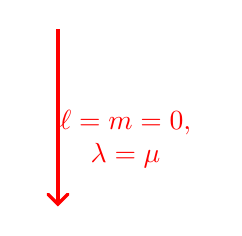
\begin{tikzpicture}
			\draw[->,>=angle 90,color=red,style=very thick] (2.0,4.8) -- node{} (2.0,2.55);
			\node at (2.8,3.4) {\color{red}{\textnormal{ $\begin{array}[]{c}\ell=m=0,\\ \lambda=\mu \end{array}$}}};
		\end{tikzpicture}
	\end{textblock*}
	\begin{textblock*}{\textwidth}(3.99cm,1.7cm)
	  	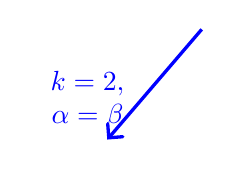
\begin{tikzpicture}
			\draw[->,>=angle 90,color=blue,style=very thick] (1.0,1.0) -- node{} (-0.2,-0.4);
			\node at (-0.45,0.1) {\color{blue}{\normalfont{$\begin{array}[]{c}
				k=2,\\
			\alpha=\beta
		\end{array}$}}};
		\end{tikzpicture}
	\end{textblock*}
	\begin{textblock*}{0.5\textwidth}(-0.4cm,3.14cm)
		 {
			\begin{tcolorbox}[colback=green!10!white,colframe=green]
				\vspace{-0.5cm}
		\begin{equation*}
			\kern-0.4cm
			\begin{array}[]{c}
				\displaystyle\iint\displaylimits_{\kern0.2cm [-1,1]^2}\kern-0.3cm | s - t |^{2 \nu}\kern-0.05cm (1 - s^2)^{\lambda - \frac{1}{2}}
			\kern-0.05cm(1 - t^2)^{\lambda - \frac{1}{2}}d s d t\\
			=\mypgf
			\end{array}
		\end{equation*}
			     \end{tcolorbox}
		}
	\end{textblock*}
	\begin{textblock*}{0.5\textwidth}(0.5\textwidth,1.35cm)
    			\setulcolor{Blue}
	\end{textblock*}
	\begin{textblock*}{0.5\textwidth}(0.635\textwidth,-2.8cm)
			  \begin{tikzpicture}[scale=0.4]
				\draw[color=black] (-0.2,0.0) rectangle (2.2,-0.5);
\node at (1.0,-0.25) {\color{black}{\tiny W'10:\color{blue}{4}}};

\draw[color=red] (2.4,0.0) rectangle (4.4,-0.5);
\node at (3.45,-0.25) {\color{red}{\tiny 命題 2:\color{blue}{4}}};

\draw[color=black] (4.6,0.0) rectangle (7.6,-0.5);
\node at (6.1,-0.25) {\color{black}{\tiny T-V'03:\color{blue}{3}}};

\draw[color=black] (8.5,0.0) rectangle (11.25,-0.5);
\node at (9.85,-0.25) {\color{black}{\tiny D-F'85:\color{blue}{4}}};

\draw[color=red] (2.1,-2.0) rectangle (4.3,-2.5);
\node at (3.2,-2.25) {\color{red}{\tiny 命題 1$'$:\color{blue}{3}}};

\filldraw[color=red,pattern color=red,pattern=north east lines] (3.2,-4.0) circle(0.3);
\node at (3.85,-4.0) {\color{blue}{3}};

\fill[color=black] (1.5,-6.0) circle(0.1);
\node at (1.95,-6.0) {\color{blue}{2}};

\fill[color=green] (3.2,-6.0) circle(0.3);
\node at (3.6500000000000004,-6.0) {\color{blue}{2}};

\fill[color=black] (5.85,-6.0) circle(0.1);
\node at (6.3,-6.0) {\color{blue}{2}};

\fill[color=black] (8.9,-6.0) circle(0.1);
\node at (9.35,-6.0) {\color{blue}{2}};


\draw[->,>=angle 90,color=black] (2.0,-0.5) -- node {} (5.0,-2.0) ;%War -> S
\draw[->,>=angle 90,style=very thick,color=red] (3.2,-0.5) -- node {} (3.2,-2.0) ; %P2 -> P3
\draw[->,>=angle 90,color=black] (5.1,-0.5) -- node {} (5.85,-2.0) ; %TV -> S
\draw[->,>=angle 90,color=black] (8.5,-0.5) -- node {} (6.605,-2.0) ; % DF -> S
\draw[->,>=angle 90,style=very thick,color=red] (3.2,-2.5) -- node {} (3.2000000000000006,-3.7) ; % P3 -> P3'
\draw[->,>=angle 90,color=black] (1.0,-0.5) -- node {} (1.490946425395748,-5.90041067935323) ; %W -> W'
\draw[->,>=angle 90,color=black] (3.0057054739713385,-4.2285817953278375) -- node {} (1.5573628100792203,-5.93251434108327) ;%P3' -> W'
\draw[->,>=angle 90,style=very thick,color=red] (3.2,-4.3) -- node {} (3.2,-5.714999999999999) ;%P3' -> S'
\draw[->,>=angle 90,color=black] (3.4394567450999696,-4.180722071773562) -- node {} (5.777393604812446,-5.9452027206131675) ;%P3' -> DF'
\draw[->,>=angle 90,color=black] (3.4830799946398643,-4.099326313908724) -- node {} (8.810326217188193,-5.968535514802874) ;%P3' -> TV'
\draw[->,>=angle 90,style=very thick,color=blue] (5.34,-2.5) -- node {} (3.35649415847905,-5.74405160996417) ;%S -> S'
\draw[->,>=angle 90,color=black] (9.6,-0.5) -- node {}  (8.92466,-5.90309);%DF -> DF'
\draw[->,>=angle 90,color=black] (6.5,-0.5) -- node {} (5.88,-5.9048) ;%TV -> TV'

\draw[color=blue,fill=white] (4.8,-2.0) rectangle (6.9,-2.5);
\node at (5.85,-2.25) {\color{blue}{\tiny S'44:\color{blue}{3}}};

				\end{tikzpicture}
				%\caption{A gull}
	\end{textblock*}
	{
	\begin{textblock*}{0.5\textwidth}(-0.2cm,-2.4cm)
    			\setulcolor{Red}
			\begin{block}{{\ul{{\mbox{命題}} $1'$}}}
		{
		\begin{equation*}
			\kern-0.4cm
			\begin{array}[]{c}
				\displaystyle\iint\displaylimits_{\kern0.2cm [-1,1]^2}\kern-0.3cm | s - t |^{2 \nu}\kern-0.05cm (1 - s^2)^{\lambda - \frac{1}{2}}
			\kern-0.05cm(1 - t^2)^{\mu - \frac{1}{2}} C_\ell^{\lambda} (s) C_m^{\mu} (t) d s d t\\
			=\mypgf
			\end{array}
		\end{equation*}
		}
	\end{block}
	\end{textblock*}
	}
\end{frame}
\begin{frame}[fragile]
\begin{tikzpicture}
\draw[color=blue] (-0.2,0.0) rectangle (2.2,-0.5);
\node at (1.0,-0.25) {\color{blue}{\scriptsize Warnaar'10: \color{blue}{4}}};

\draw[color=red] (2.4,0.0) rectangle (4.4,-0.5);
\node at (3.45,-0.25) {\color{red}{\scriptsize 命題 2: \color{blue}{4}}};

\draw[color=black] (4.6,0.0) rectangle (7.6,-0.5);
\node at (6.1,-0.25) {\color{black}{\scriptsize Tarasov-Varchenko'03: \color{blue}{3}}};

\draw[color=black] (8.5,0.0) rectangle (11.25,-0.5);
\node at (9.85,-0.25) {\color{black}{\scriptsize Dotsenko-Fateev'85: \color{blue}{4}}};

\draw[color=red] (2.1,-2.0) rectangle (4.3,-2.5);
\node at (3.2,-2.25) {\color{red}{\scriptsize 命題 1$'$: \color{blue}{3}}};

\filldraw[color=red,pattern color=red,pattern=north east lines] (3.2,-4.0) circle(0.3);
\node at (3.85,-4.0) {\color{blue}{3}};

\fill[color=green] (1.5,-6.0) circle(0.3);
\node at (1.95,-6.0) {\color{blue}{2}};

\fill[color=black] (3.2,-6.0) circle(0.1);
\node at (3.6500000000000004,-6.0) {\color{blue}{2}};

\fill[color=black] (5.85,-6.0) circle(0.1);
\node at (6.3,-6.0) {\color{blue}{2}};

\fill[color=black] (8.9,-6.0) circle(0.1);
\node at (9.35,-6.0) {\color{blue}{2}};


\draw[->,>=angle 90,color=black] (2.0,-0.5) -- node {} (5.0,-2.0) ;%War -> S
\draw[->,>=angle 90,color=red,style=very thick] (3.2,-0.5) -- node {} (3.2,-2.0) ; %P2 -> P3
\draw[->,>=angle 90,color=black] (5.1,-0.5) -- node {} (5.85,-2.0) ; %TV -> S
\draw[->,>=angle 90,color=black] (8.5,-0.5) -- node {} (6.605,-2.0) ; % DF -> S
\draw[->,>=angle 90,color=red,style=very thick] (3.2,-2.5) -- node {} (3.2000000000000006,-3.7) ; % P3 -> P3'
\draw[->,>=angle 90,color=blue,style=very thick] (1.0,-0.5) -- node {} (1.4719,-5.7) ; %W -> W'
\draw[->,>=angle 90,color=red,style=very thick] (3.00,-4.23) -- node {} (1.68,-5.77) ;%P3' -> W'
\draw[->,>=angle 90,color=black] (3.2,-4.3) -- node {} (3.2,-5.914999999999999) ;%P3' -> S'
\draw[->,>=angle 90,color=black] (3.4394567450999696,-4.180722071773562) -- node {} (5.777393604812446,-5.9452027206131675) ;%P3' -> DF'
\draw[->,>=angle 90,color=black] (3.4830799946398643,-4.099326313908724) -- node {} (8.810326217188193,-5.968535514802874) ;%P3' -> TV'
\draw[->,>=angle 90,color=black] (5.34,-2.5) -- node {} (3.252164719493017,-5.914683869988056) ;%S -> S'
\draw[->,>=angle 90,color=black] (9.6,-0.5) -- node {}  (8.92466,-5.90309);%DF -> DF'
\draw[->,>=angle 90,color=black] (6.5,-0.5) -- node {} (5.88,-5.9048) ;%TV -> TV'

\draw[color=black,fill=white] (4.8,-2.0) rectangle (6.9,-2.5);
\node at (5.85,-2.25) {\color{black}{\scriptsize Selberg'44: \color{black}{3}}};

\end{tikzpicture}
ここで{\color{blue}{青い数字}}は連続パラメータの個数を表す.
\end{frame}
\begin{frame}[fragile]%frame Warnaar
	
	\begin{textblock*}{0.5\textwidth}(-0.2cm,-2.65cm)
    			\setulcolor{Blue}
	\end{textblock*}
	\begin{textblock*}{\textwidth}(7.99cm,2.75cm)
	  	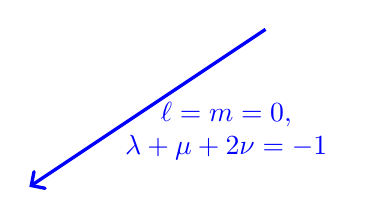
\begin{tikzpicture}
			\draw[->,>=angle 90,color=blue,style=very thick] (1.0,1.0) -- node{} (-2.0,-1.0);
			\node at (0.5,-0.3) {\color{blue}{$
				\begin{array}[]{c}
					\ell=m=0,\\
				\lambda+\mu+2\nu=-1
				\end{array}
		$}};
		\end{tikzpicture}
	\end{textblock*}
	\begin{textblock*}{0.7\textwidth}(-0.4cm,3.7cm)
		 {
			\begin{tcolorbox}[colback=green!10!white,colframe=green]
				\vspace{-0.7cm}
		\begin{equation*}
			\kern-0.4cm
			\begin{array}[]{c}
				\left(\displaystyle\iint\displaylimits_{\scalebox{0.7}{$\begin{array}[]{c}
					[0,1]^2\\t<s
				\end{array}$}}+\frac{\sin(\pi\alpha_1)}{\sin(\pi\alpha_2)}\displaystyle\iint\displaylimits_{\scalebox{0.7}{$\begin{array}[]{c}
					[0,1]^2\\t>s
				\end{array}$}} \right)(t(1-t))^{\mu - \frac{1}{2}}  (s(1-s))^{\lambda - \frac{1}{2}}  | t - s |^{2\nu} d s d t
			\\=\mypgf
			\end{array}
		\end{equation*}
				\vspace{-0.7cm}
			     \end{tcolorbox}
		}
	\end{textblock*}
	\begin{textblock*}{\textwidth}(0.7cm,3.1cm)
	  	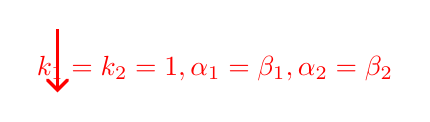
\begin{tikzpicture}
			\draw[->,>=angle 90,color=red,style=very thick] (2.0,2.8) -- node{} (2.0,2.0);
			\node at (4.0,2.3) {\color{red}{$k_1=k_2=1,\alpha_1=\beta_1,\alpha_2=\beta_2$}};
		\end{tikzpicture}
	\end{textblock*}
	\begin{textblock*}{0.5\textwidth}(0.635\textwidth,-2.8cm)
			  \begin{tikzpicture}[scale=0.4]
				\draw[color=blue] (-0.2,0.0) rectangle (2.2,-0.5);
\node at (1.0,-0.25) {\color{blue}{\tiny W'10:\color{blue}{4}}};

\draw[color=red] (2.4,0.0) rectangle (4.4,-0.5);
\node at (3.45,-0.25) {\color{red}{\tiny 命題 2:\color{blue}{4}}};

\draw[color=black] (4.6,0.0) rectangle (7.6,-0.5);
\node at (6.1,-0.25) {\color{black}{\tiny T-V'03:\color{blue}{3}}};

\draw[color=black] (8.5,0.0) rectangle (11.25,-0.5);
\node at (9.85,-0.25) {\color{black}{\tiny D-F'85:\color{blue}{4}}};

\draw[color=red] (2.1,-2.0) rectangle (4.3,-2.5);
\node at (3.2,-2.25) {\color{red}{\tiny 命題 1$'$:\color{blue}{3}}};

\filldraw[color=red,pattern color=red,pattern=north east lines] (3.2,-4.0) circle(0.3);
\node at (3.85,-4.0) {\color{blue}{3}};

\fill[color=green] (1.5,-6.0) circle(0.3);
\node at (1.95,-6.0) {\color{blue}{2}};

\fill[color=black] (3.2,-6.0) circle(0.1);
\node at (3.6500000000000004,-6.0) {\color{blue}{2}};

\fill[color=black] (5.85,-6.0) circle(0.1);
\node at (6.3,-6.0) {\color{blue}{2}};

\fill[color=black] (8.9,-6.0) circle(0.1);
\node at (9.35,-6.0) {\color{blue}{2}};


\draw[->,>=angle 90,color=black] (2.0,-0.5) -- node {} (5.0,-2.0) ;%War -> S
\draw[->,>=angle 90,color=red,style=very thick] (3.2,-0.5) -- node {} (3.2,-2.0) ; %P2 -> P3
\draw[->,>=angle 90,color=black] (5.1,-0.5) -- node {} (5.85,-2.0) ; %TV -> S
\draw[->,>=angle 90,color=black] (8.5,-0.5) -- node {} (6.605,-2.0) ; % DF -> S
\draw[->,>=angle 90,color=red,style=very thick] (3.2,-2.5) -- node {} (3.2000000000000006,-3.7) ; % P3 -> P3'
\draw[->,>=angle 90,color=blue,style=very thick] (1.0,-0.5) -- node {} (1.4719,-5.7) ; %W -> W'
\draw[->,>=angle 90,color=red,style=very thick] (3.00,-4.23) -- node {} (1.68,-5.77) ;%P3' -> W'
\draw[->,>=angle 90,color=black] (3.2,-4.3) -- node {} (3.2,-5.914999999999999) ;%P3' -> S'
\draw[->,>=angle 90,color=black] (3.4394567450999696,-4.180722071773562) -- node {} (5.777393604812446,-5.9452027206131675) ;%P3' -> DF'
\draw[->,>=angle 90,color=black] (3.4830799946398643,-4.099326313908724) -- node {} (8.810326217188193,-5.968535514802874) ;%P3' -> TV'
\draw[->,>=angle 90,color=black] (5.34,-2.5) -- node {} (3.252164719493017,-5.914683869988056) ;%S -> S'
\draw[->,>=angle 90,color=black] (9.6,-0.5) -- node {}  (8.92466,-5.90309);%DF -> DF'
\draw[->,>=angle 90,color=black] (6.5,-0.5) -- node {} (5.88,-5.9048) ;%TV -> TV'

\draw[color=black,fill=white] (4.8,-2.0) rectangle (6.9,-2.5);
\node at (5.85,-2.25) {\color{black}{\tiny S'44:\color{black}{3}}};

				\end{tikzpicture}
	\end{textblock*}
	\begin{textblock*}{0.5\textwidth}(0.52\textwidth,0.75cm)
    			\setulcolor{Red}
			\begin{block}{\ul{{\mbox{命題}} $1'$}}
		{
		\begin{equation*}
			\kern-1.1cm
			\begin{array}[]{c}
				\displaystyle\iint\displaylimits_{\kern0.2cm [-1,1]^2}\kern-0.3cm | s - t |^{2 \nu}\kern-0.05cm (1 - s^2)^{\lambda - \frac{1}{2}}
			\kern-0.05cm(1 - t^2)^{\mu - \frac{1}{2}} C_\ell^{\lambda} (s) C_m^{\mu} (t) d s d t\kern-1cm\\
			=\mypgf
			\end{array}
		\end{equation*}
		}
	\end{block}
	\end{textblock*}
\end{frame}
\begin{frame}[fragile]
\begin{tikzpicture}
\draw[color=black] (-0.2,0.0) rectangle (2.2,-0.5);
\node at (1.0,-0.25) {\color{black}{\scriptsize Warnaar'10: \color{blue}{4}}};

\draw[color=red] (2.4,0.0) rectangle (4.4,-0.5);
\node at (3.45,-0.25) {\color{red}{\scriptsize 命題 2: \color{blue}{4}}};

\draw[color=blue] (4.5,0.0) rectangle (7.7,-0.5);
\node at (6.1,-0.25) {\color{blue}{\scriptsize Tarasov-Varchenko'03: \color{blue}{3}}};

\draw[color=black] (8.4,0.0) rectangle (11.35,-0.5);
\node at (9.85,-0.25) {\color{black}{\scriptsize Dotsenko-Fateev'85: \color{blue}{4}}};

\draw[color=red] (2.1,-2.0) rectangle (4.3,-2.5);
\node at (3.2,-2.25) {\color{red}{\scriptsize 命題 1$'$: \color{blue}{3}}};

\filldraw[color=red,pattern color=red,pattern=north east lines] (3.2,-4.0) circle(0.3);
\node at (3.85,-4.0) {\color{blue}{3}};

\fill[color=black] (1.5,-6.0) circle(0.1);
\node at (1.95,-6.0) {\color{blue}{2}};

\fill[color=black] (3.2,-6.0) circle(0.1);
\node at (3.6500000000000004,-6.0) {\color{blue}{2}};

\fill[color=green] (5.85,-6.0) circle(0.3);
\node at (6.3,-6.0) {\color{blue}{2}};

\fill[color=black] (8.9,-6.0) circle(0.1);
\node at (9.35,-6.0) {\color{blue}{2}};


\draw[->,>=angle 90,color=black] (2.0,-0.5) -- node {} (5.0,-2.0) ;%War -> S
\draw[->,>=angle 90,style=very thick,color=red] (3.2,-0.5) -- node {} (3.2,-2.0) ; %P2 -> P3
\draw[->,>=angle 90,color=black] (5.1,-0.5) -- node {} (5.85,-2.0) ; %TV -> S
\draw[->,>=angle 90,color=black] (8.5,-0.5) -- node {} (6.605,-2.0) ; % DF -> S
\draw[->,>=angle 90,style=very thick,color=red] (3.2,-2.5) -- node {} (3.2000000000000006,-3.7) ; % P3 -> P3'
\draw[->,>=angle 90,color=black] (1.0,-0.5) -- node {} (1.490946425395748,-5.90041067935323) ; %W -> W'
\draw[->,>=angle 90,color=black] (3.0057054739713385,-4.2285817953278375) -- node {} (1.5573628100792203,-5.93251434108327) ;%P3' -> W'
\draw[->,>=angle 90,color=black] (3.2,-4.3) -- node {} (3.2,-5.914999999999999) ;%P3' -> S'
\draw[->,>=angle 90,color=red,style=very thick] (3.44,-4.18) -- node {} (5.6174,-5.82446) ;%P3' -> TV'
\draw[->,>=angle 90,color=black,color=black] (3.48,-4.099) -- node {} (8.81,-5.9685) ;%P3' -> DF'
\draw[->,>=angle 90,color=black] (5.34,-2.5) -- node {} (3.252164719493017,-5.914683869988056) ;%S -> S'
\draw[->,>=angle 90,color=black] (5.34,-2.5) -- node {} (3.252164719493017,-5.914683869988056) ;%S -> S'
\draw[->,>=angle 90,color=black] (9.6,-0.5) -- node {}  (8.92466,-5.90309);%DF -> DF'
\draw[->,>=angle 90,color=blue,style=very thick] (6.5,-0.5) -- node {} (5.90279,-5.70610) ;%TV -> TV'

\draw[color=black,fill=white] (4.8,-2.0) rectangle (6.9,-2.5);
\node at (5.85,-2.25) {\color{black}{\scriptsize Selberg'44: \color{black}{3}}};

\end{tikzpicture}
ここで{\color{blue}{青い数字}}は連続パラメータの個数を表す.
\end{frame}
\begin{frame}[fragile]%frame TV
	
	\begin{textblock*}{\textwidth}(1cm,0.8cm)
	  	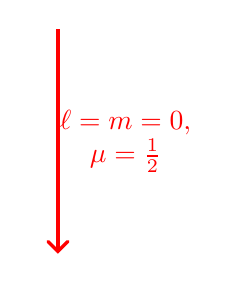
\begin{tikzpicture}
			\draw[->,>=angle 90,color=red,style=very thick] (2.0,4.8) -- node{} (2.0,1.95);
			\node at (2.8,3.4) {\color{red}{\textnormal{ $\begin{array}[]{c}\ell=m=0,\\ \mu=\frac{1}{2} \end{array}$}}};
		\end{tikzpicture}
	\end{textblock*}
	\begin{textblock*}{\textwidth}(3.89cm,1.7cm)
	  	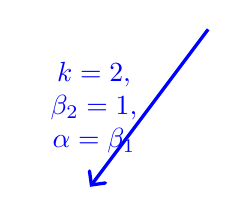
\begin{tikzpicture}
			\draw[->,>=angle 90,color=blue,style=very thick] (1.0,1.0) -- node{} (-0.5,-1.0);
			\node at (-0.45,0.0) {\color{blue}{\normalfont{$\begin{array}[]{c}
				k=2,\\
				\beta_2=1,\\
				\alpha=\beta_1
		\end{array}$}}};
		\end{tikzpicture}
	\end{textblock*}
	\begin{textblock*}{0.5\textwidth}(-0.4cm,3.7cm)
		 {
			\begin{tcolorbox}[colback=green!10!white,colframe=green]
				\vspace{-0.5cm}
			\begin{equation*}
				\kern-0.6cm
				\begin{array}[]{c}
					
				\displaystyle\iint\displaylimits_{\begin{array}[]{c}
				(s, t) \in [0, 1]^2\\t<s
			\end{array}} s^{\lambda - \frac{1}{2}} (1 - s)^{\lambda-\frac{1}{2}} \myabs{s-t}^{2\nu} d s d t\\
			=\mypgf
				\end{array}
				\vspace{-0.3cm}
			\end{equation*}

			     \end{tcolorbox}
		}
	\end{textblock*}
	\begin{textblock*}{0.5\textwidth}(0.515\textwidth,0.1cm)
    			\setulcolor{Blue}
	\end{textblock*}
	\begin{textblock*}{0.5\textwidth}(0.635\textwidth,-2.8cm)
			  \begin{tikzpicture}[scale=0.4]
				\draw[color=black] (-0.2,0.0) rectangle (2.2,-0.5);
\node at (1.0,-0.25) {\color{black}{\tiny W'10:\color{blue}{4}}};

\draw[color=red] (2.4,0.0) rectangle (4.4,-0.5);
\node at (3.45,-0.25) {\color{red}{\tiny 命題 2:\color{blue}{4}}};

\draw[color=blue] (4.6,0.0) rectangle (7.6,-0.5);
\node at (6.1,-0.25) {\color{blue}{\tiny T-V'03:\color{blue}{3}}};

\draw[color=black] (8.5,0.0) rectangle (11.25,-0.5);
\node at (9.85,-0.25) {\color{black}{\tiny D-F'85:\color{blue}{4}}};

\draw[color=red] (2.1,-2.0) rectangle (4.3,-2.5);
\node at (3.2,-2.25) {\color{red}{\tiny 命題 1$'$:\color{blue}{3}}};

\filldraw[color=red,pattern color=red,pattern=north east lines] (3.2,-4.0) circle(0.3);
\node at (3.85,-4.0) {\color{blue}{3}};

\fill[color=black] (1.5,-6.0) circle(0.1);
\node at (1.95,-6.0) {\color{blue}{2}};

\fill[color=black] (3.2,-6.0) circle(0.1);
\node at (3.6500000000000004,-6.0) {\color{blue}{2}};

\fill[color=green] (5.85,-6.0) circle(0.3);
\node at (6.3,-6.0) {\color{blue}{2}};

\fill[color=black] (8.9,-6.0) circle(0.1);
\node at (9.35,-6.0) {\color{blue}{2}};


\draw[->,>=angle 90,color=black] (2.0,-0.5) -- node {} (5.0,-2.0) ;%War -> S
\draw[->,>=angle 90,style=very thick,color=red] (3.2,-0.5) -- node {} (3.2,-2.0) ; %P2 -> P3
\draw[->,>=angle 90,color=black] (5.1,-0.5) -- node {} (5.85,-2.0) ; %TV -> S
\draw[->,>=angle 90,color=black] (8.5,-0.5) -- node {} (6.605,-2.0) ; % DF -> S
\draw[->,>=angle 90,style=very thick,color=red] (3.2,-2.5) -- node {} (3.2000000000000006,-3.7) ; % P3 -> P3'
\draw[->,>=angle 90,color=black] (1.0,-0.5) -- node {} (1.490946425395748,-5.90041067935323) ; %W -> W'
\draw[->,>=angle 90,color=black] (3.0057054739713385,-4.2285817953278375) -- node {} (1.5573628100792203,-5.93251434108327) ;%P3' -> W'
\draw[->,>=angle 90,color=black] (3.2,-4.3) -- node {} (3.2,-5.914999999999999) ;%P3' -> S'
\draw[->,>=angle 90,color=red,style=very thick] (3.44,-4.18) -- node {} (5.6174,-5.82446) ;%P3' -> TV'
\draw[->,>=angle 90,color=black,color=black] (3.48,-4.099) -- node {} (8.81,-5.9685) ;%P3' -> DF'
\draw[->,>=angle 90,color=black] (5.34,-2.5) -- node {} (3.252164719493017,-5.914683869988056) ;%S -> S'
\draw[->,>=angle 90,color=black] (5.34,-2.5) -- node {} (3.252164719493017,-5.914683869988056) ;%S -> S'
\draw[->,>=angle 90,color=black] (9.6,-0.5) -- node {}  (8.92466,-5.90309);%DF -> DF'
\draw[->,>=angle 90,color=blue,style=very thick] (6.5,-0.5) -- node {} (5.90279,-5.70610) ;%TV -> TV'

\draw[color=black,fill=white] (4.8,-2.0) rectangle (6.9,-2.5);
\node at (5.85,-2.25) {\color{black}{\tiny S'44:\color{black}{3}}};

				\end{tikzpicture}
				%\caption{A gull}
	\end{textblock*}
	{
	\begin{textblock*}{0.5\textwidth}(-0.2cm,-2.4cm)
    			\setulcolor{Red}
			\begin{block}{{\ul{{\mbox{命題}} $1'$}}}
		{
		\begin{equation*}
			\kern-0.4cm
			\begin{array}[]{c}
				\displaystyle\iint\displaylimits_{\kern0.2cm [-1,1]^2}\kern-0.3cm | s - t |^{2 \nu}\kern-0.05cm (1 - s^2)^{\lambda - \frac{1}{2}}
			\kern-0.05cm(1 - t^2)^{\mu - \frac{1}{2}} C_\ell^{\lambda} (s) C_m^{\mu} (t) d s d t\\
			=\mypgf
			\end{array}
		\end{equation*}
		}
	\end{block}
	\end{textblock*}
	}
\end{frame}
\begin{frame}[fragile]
\begin{tikzpicture}
\draw[color=black] (-0.2,0.0) rectangle (2.2,-0.5);
\node at (1.0,-0.25) {\color{black}{\scriptsize Warnaar'10: \color{blue}{4}}};

\draw[color=red] (2.4,0.0) rectangle (4.4,-0.5);
\node at (3.45,-0.25) {\color{red}{\scriptsize 命題 2: \color{blue}{4}}};

\draw[color=black] (4.5,0.0) rectangle (7.7,-0.5);
\node at (6.1,-0.25) {\color{black}{\scriptsize Tarasov-Varchenko'03: \color{black}{3}}};

\draw[color=blue] (8.4,0.0) rectangle (11.35,-0.5);
\node at (9.85,-0.25) {\color{blue}{\scriptsize Dotsenko-Fateev'85: \color{blue}{4}}};

\draw[color=red] (2.1,-2.0) rectangle (4.3,-2.5);
\node at (3.2,-2.25) {\color{red}{\scriptsize 命題 1$'$: \color{blue}{3}}};

\filldraw[color=red,pattern color=red,pattern=north east lines] (3.2,-4.0) circle(0.3);
\node at (3.85,-4.0) {\color{blue}{3}};

\fill[color=black] (1.5,-6.0) circle(0.1);
\node at (1.95,-6.0) {\color{blue}{2}};

\fill[color=black] (3.2,-6.0) circle(0.1);
\node at (3.6500000000000004,-6.0) {\color{blue}{2}};

\fill[color=black] (5.85,-6.0) circle(0.1);
\node at (6.3,-6.0) {\color{blue}{2}};

\fill[color=green] (8.9,-6.0) circle(0.3);
\node at (9.35,-6.0) {\color{blue}{2}};


\draw[->,>=angle 90,color=black] (2.0,-0.5) -- node {} (5.0,-2.0) ;%War -> S
\draw[->,>=angle 90,style=very thick,color=red] (3.2,-0.5) -- node {} (3.2,-2.0) ; %P2 -> P3
\draw[->,>=angle 90,color=black] (5.1,-0.5) -- node {} (5.85,-2.0) ; %TV -> S
\draw[->,>=angle 90,color=black] (8.5,-0.5) -- node {} (6.605,-2.0) ; % DF -> S
\draw[->,>=angle 90,style=very thick,color=red] (3.2,-2.5) -- node {} (3.2000000000000006,-3.7) ; % P3 -> P3'
\draw[->,>=angle 90,color=black] (1.0,-0.5) -- node {} (1.490946425395748,-5.90041067935323) ; %W -> W'
\draw[->,>=angle 90,color=black] (3.0057054739713385,-4.2285817953278375) -- node {} (1.5573628100792203,-5.93251434108327) ;%P3' -> W'
\draw[->,>=angle 90,color=black] (3.2,-4.3) -- node {} (3.2,-5.914999999999999) ;%P3' -> S'
\draw[->,>=angle 90,color=black] (3.44,-4.18) -- node {} (5.777393604812446,-5.9452027206131675) ;%P3' -> TV'
\draw[->,>=angle 90,color=red,style=very thick] (3.48,-4.099) -- node {} (8.621,-5.9) ;%P3' -> DF'
\draw[->,>=angle 90,color=black] (5.34,-2.5) -- node {} (3.252164719493017,-5.914683869988056) ;%S -> S'
\draw[->,>=angle 90,color=blue,style=very thick] (9.6,-0.5) -- node {}  (8.9494,-5.70463);%DF -> DF'
\draw[->,>=angle 90,color=black] (6.5,-0.5) -- node {} (5.88,-5.9048) ;%TV -> TV'

\draw[color=black,fill=white] (4.8,-2.0) rectangle (6.9,-2.5);
\node at (5.85,-2.25) {\color{black}{\scriptsize Selberg'44: \color{black}{3}}};

\end{tikzpicture}
ここで{\color{blue}{青い数字}}は連続パラメータの個数を表す.
\end{frame}
\begin{frame}[fragile]%frame DF
	
	\begin{textblock*}{\textwidth}(1cm,0.8cm)
	  	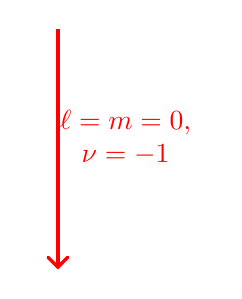
\begin{tikzpicture}
			\draw[->,>=angle 90,color=red,style=very thick] (2.0,4.8) -- node{} (2.0,1.75);
			\node at (2.8,3.4) {\color{red}{\textnormal{ $\begin{array}[]{c}\ell=m=0,\\ \nu=-1\end{array}$}}};
		\end{tikzpicture}
	\end{textblock*}
	\begin{textblock*}{\textwidth}(3.89cm,1.9cm)
	  	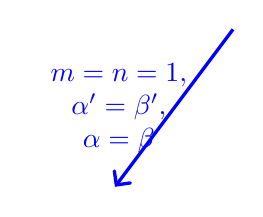
\begin{tikzpicture}
			\draw[->,>=angle 90,color=blue,style=very thick] (1.0,1.0) -- node{} (-0.5,-1.0);
			\node at (-0.45,0.0) {\color{blue}{\normalfont{$\begin{array}[]{c}
				m=n=1,\\
				\alpha'=\beta',\\
				\alpha=\beta
		\end{array}$}}};
		\end{tikzpicture}
	\end{textblock*}
	\begin{textblock*}{0.5\textwidth}(-0.4cm,3.9cm)
		 {
			\begin{tcolorbox}[colback=green!10!white,colframe=green]
				\vspace{-0.5cm}
			\begin{equation*}
				\kern-0.6cm
				\begin{array}{c}
				\displaystyle\iint\displaylimits_{(t, \tau) \in [0, 1]^2} t^{\alpha'} (1 - t)^{\alpha'} \tau^{\alpha} (1
				- \tau)^{\alpha} | t - \tau |^{- 2} dtd\tau\\
			=\mypgf
				\end{array}
				\vspace{-0.3cm}
			\end{equation*}

			     \end{tcolorbox}
		}
	\end{textblock*}
	\begin{textblock*}{0.5\textwidth}(0.515\textwidth,-0.2cm)
    			\setulcolor{Blue}
		\begin{fact*}[{\ul{Dotsenko-Fateev'85}}]
			{
		\begin{equation*}
			\kern-0.25cm
			\begin{array}{c}
				\frac{1}{n!m!}
				\kern-1.45cm
				\displaystyle\bigintssss_{\mbox{$\kern1.0cm(t,\tau)\kern-0.1cm\in\kern-0.1cm [0, 1]^{k_1+k_2}$}} \kern-1.35cm
   \Pi^{\alpha', \beta'} (t)
  \Pi^{\alpha, \beta} (\tau) \Delta^{2 \rho'}(t) \Delta^{2 \rho}(\tau)
  \Delta^{- 2} (t, \tau) dtd\tau \\
				      \end{array}\end{equation*}
			\vspace{-0.5cm}
		\begin{equation*}
			\kern-0.29cm
			\begin{array}{c}
					        = \mypgf,\\
					  \mbox{ここで  }\textstyle\prod^{\alpha - 1,
					  \beta_1 - 1} (t):=\displaystyle\prod_{i=1}^{k_1}t_i^{\alpha-1}(1-t_i)^{\beta_1-1},\\
					  \Delta^{2\gamma}(t):=\displaystyle\prod_{1\le i<j\le k_1 }\kern-0.2cm\myabs{t_i}^{2\gamma}, \Delta^\gamma(t,s):=\displaystyle\prod\displaylimits_{i,j=1}^{k_1,k_2}
					  \myabs{t_i-s_j}^{\gamma}\kern-0.1cm,\\
					  \\
  \alpha' = - \rho' \alpha, \beta' = - \rho' \beta, \rho' \rho = 1,\\
  \tmop{Re} (\rho) < 0, \quad \tmop{Re} (\alpha), \tmop{Re} (\beta) > (n - 1)
  + | \tmop{Re} (\rho) | (m - 1).
			\end{array}
			\end{equation*}
			\vspace{-0.29cm}
				}
		\end{fact*}
	\end{textblock*}
	\begin{textblock*}{0.5\textwidth}(0.635\textwidth,-2.8cm)
			  \begin{tikzpicture}[scale=0.4]
				\draw[color=black] (-0.2,0.0) rectangle (2.2,-0.5);
\node at (1.0,-0.25) {\color{black}{\tiny W'10:\color{blue}{4}}};

\draw[color=red] (2.4,0.0) rectangle (4.4,-0.5);
\node at (3.45,-0.25) {\color{red}{\tiny 命題 2:\color{blue}{4}}};

\draw[color=black] (4.6,0.0) rectangle (7.6,-0.5);
\node at (6.1,-0.25) {\color{black}{\tiny T-V'03:\color{black}{3}}};

\draw[color=blue] (8.5,0.0) rectangle (11.25,-0.5);
\node at (9.85,-0.25) {\color{blue}{\tiny D-F'85:\color{blue}{4}}};

\draw[color=red] (2.1,-2.0) rectangle (4.3,-2.5);
\node at (3.2,-2.25) {\color{red}{\tiny 命題 1$'$:\color{blue}{3}}};

\filldraw[color=red,pattern color=red,pattern=north east lines] (3.2,-4.0) circle(0.3);
\node at (3.85,-4.0) {\color{blue}{3}};

\fill[color=black] (1.5,-6.0) circle(0.1);
\node at (1.95,-6.0) {\color{blue}{2}};

\fill[color=black] (3.2,-6.0) circle(0.1);
\node at (3.6500000000000004,-6.0) {\color{blue}{2}};

\fill[color=black] (5.85,-6.0) circle(0.1);
\node at (6.3,-6.0) {\color{blue}{2}};

\fill[color=green] (8.9,-6.0) circle(0.3);
\node at (9.35,-6.0) {\color{blue}{2}};


\draw[->,>=angle 90,color=black] (2.0,-0.5) -- node {} (5.0,-2.0) ;%War -> S
\draw[->,>=angle 90,style=very thick,color=red] (3.2,-0.5) -- node {} (3.2,-2.0) ; %P2 -> P3
\draw[->,>=angle 90,color=black] (5.1,-0.5) -- node {} (5.85,-2.0) ; %TV -> S
\draw[->,>=angle 90,color=black] (8.5,-0.5) -- node {} (6.605,-2.0) ; % DF -> S
\draw[->,>=angle 90,style=very thick,color=red] (3.2,-2.5) -- node {} (3.2000000000000006,-3.7) ; % P3 -> P3'
\draw[->,>=angle 90,color=black] (1.0,-0.5) -- node {} (1.490946425395748,-5.90041067935323) ; %W -> W'
\draw[->,>=angle 90,color=black] (3.0057054739713385,-4.2285817953278375) -- node {} (1.5573628100792203,-5.93251434108327) ;%P3' -> W'
\draw[->,>=angle 90,color=black] (3.2,-4.3) -- node {} (3.2,-5.914999999999999) ;%P3' -> S'
\draw[->,>=angle 90,color=black] (3.44,-4.18) -- node {} (5.777393604812446,-5.9452027206131675) ;%P3' -> TV'
\draw[->,>=angle 90,color=red,style=very thick] (3.48,-4.099) -- node {} (8.621,-5.9) ;%P3' -> DF'
\draw[->,>=angle 90,color=black] (5.34,-2.5) -- node {} (3.252164719493017,-5.914683869988056) ;%S -> S'
\draw[->,>=angle 90,color=blue,style=very thick] (9.6,-0.5) -- node {}  (8.9494,-5.70463);%DF -> DF'
\draw[->,>=angle 90,color=black] (6.5,-0.5) -- node {} (5.88,-5.9048) ;%TV -> TV'

\draw[color=black,fill=white] (4.8,-2.0) rectangle (6.9,-2.5);
\node at (5.85,-2.25) {\color{black}{\tiny S'44:\color{black}{3}}};

				\end{tikzpicture}
				%\caption{A gull}
	\end{textblock*}
	{
	\begin{textblock*}{0.5\textwidth}(-0.2cm,-2.4cm)
    			\setulcolor{Red}
			\begin{block}{{\ul{{\mbox{命題}} $1'$}}}
		{
		\begin{equation*}
			\kern-0.4cm
			\begin{array}[]{c}
				\displaystyle\iint\displaylimits_{\kern0.2cm [-1,1]^2}\kern-0.3cm | s - t |^{2 \nu}\kern-0.05cm (1 - s^2)^{\lambda - \frac{1}{2}}
			\kern-0.05cm(1 - t^2)^{\mu - \frac{1}{2}} C_\ell^{\lambda} (s) C_m^{\mu} (t) d s d t\\
			=\mypgf
			\end{array}
		\end{equation*}
		}
	\end{block}
	\end{textblock*}
	}
\end{frame}
\begin{frame}
	更に、系\ref{cor:int-xzy-hh}の積分に$w=s-t$変数変化し、$z=1$をとれば、
	次の公式と同等な公式(正確には、そのMellin変換)が得られる.
	\begin{fact*}[{\cite[(18)]{conte1994hermite}}]
		以下のような公式が成り立つ:
		\begin{equation}
			w_{\lambda,n}\ast w_{\lambda,k}(t)=\sqrt{\frac{(n+k)!}{2^{n+k}n!k!}}w_{\sqrt{2}\lambda,n+k}(t).
			\label{eqn:mellin-hh}
		\end{equation}
	\end{fact*}
	ここで、
	記号$w_{\lambda,n}$は\underline{Hermite-Rodriguez} 関数 \cite{yusoff2007application}
	\begin{equation*}
		w_{\lambda,n}:=\frac{1}{\sqrt{2^nn!}}H_n\left( \frac{t}{\lambda} \right)\frac{1}{\sqrt{\pi}\lambda}e^{-t^2/\lambda^2},\quad \lambda>0
	\end{equation*}
	を表す.
	%%Applying inverse Mellin transform, we arrive at the well-known formula for convolution of Hermite-Rodriguez functions.
\end{frame}
\section{証明}
\begin{frame}
	以下の述べられているメソッド1とメソッド3は最初のステップとして以下のような補題を使う:
	\begin{lemma*}[$\ell=m=0$場合に帰着]
		\begin{equation*}
			\begin{array}[]{c}
				\mbox{$\ell=m=0$特殊な場合に命題\ref{prop:int-st-gg}が成り立つ}\\[0.4cm]
				\Downarrow\\[0.4cm]
				\mbox{命題\ref{prop:int-st-gg}の一般な場合が成り立つ.}
			\end{array}
		\end{equation*}
	\end{lemma*}
	\vspace{-0.2cm}
	\begin{proof}\renewcommand{\qedsymbol}{}
		Gegenbauer多項式のロドリゲスの公式
		{\vspace{-0.2cm}\begin{equation*}
				(1-x^2)^{\alpha-\frac{1}{2}}C_n^\alpha(x)=a(\alpha,n)
				\frac{d^n}{dx^n} (1-x^2)^{n+\alpha-\frac{1}{2}},\quad a(\alpha,n)\mbox{は定数}
			\vspace{-0.2cm}\end{equation*}}
		と部分積分(integration by parts)
%%		によって、
%%				{\begin{equation}
%%			\vspace{-0.2cm}
%%					\begin{array}[]{c}
%%						\mbox{左辺}\eqref{eqn:int-st-gg}/a(\lambda,l)/a(\mu,m)\\
%%					=\iint\displaylimits_{[-1,1]^2}
%%					| s - t |^{2 \nu} \frac{\partial^l}{\partial s^l}(1-s^2)^{\lambda+l-\frac{1}{2}}\frac{\partial^m}{\partial t^m}(1-t^2)^{\mu+m-\frac{1}{2}}
%%					\\=(-1)^m(-2\nu)_{l+m}\iint\displaylimits_{[-1,1]^2}\myabs{s-t}^{2\nu-l-m}(1-s^2)^{\lambda+l-\frac{1}{2}}(1-t^2)^{\mu+m-\frac{1}{2}}.
%%					\end{array}
%%					\label{eqn:m1-1}
%%				\end{equation}}
%%				\vspace{-0.4cm}
		を用いる.
	\end{proof}
	命題\ref{prop:exp-stz-gg}の証明においても同じアイディアが適用できる.
%%	命題\ref{prop:exp-stz-gg}の積分公式の形に対して、このよう補題も成り立つ.
\end{frame}
\begin{frame}{メソッド 1 (直接)}
	
	\begin{enumerate}
		\item<2-> $\ell=m=0$ 場合を扱えばよい;
		\item<3-> 
			\begin{equation*}
				\kern-1cm
				\begin{array}[]{c}
					\mbox{
%%						\begin{tcolorbox}[colback=green!10!white,colframe=green]
							超幾何関数のオイラー積分表示
%%						\end{tcolorbox}
					}\\
					{}_2F_1\left(\begin{array}[]{c}
						a,b\\c
					\end{array};z  \right)=\frac{\Gamma(c)}{\Gamma(b)\Gamma(c-b)}\textstyle\int_0^1x^{b-1}(1-x)^{c-b-1}(1-zx)^{-a}dx,\quad\Re(c)>\Re(b)>0\\[0.2cm]
					\mybigplus\\[0.2cm]
					\mbox{超幾何関数${}_2F_1$の係数展開}\\[0.2cm]
					\scalebox{2.0}{$=$}\quad\mbox{求める積分を ${}_3F_2$ で表す}
				\end{array}
			\end{equation*}
%%			\begin{equation*}
%%				\begin{array}[]{c}
%%					\mbox{オイラー積分表示}\\[0.2cm]
%%					\mybigplus\\[0.2cm]
%%					\mbox{二次変換:\footnote{is 二次変換 correct for "quadratic transformation"?}}\quad {}_2 F_1 \left( \begin{array}{c}
%%						  1 - a, b\\
%%						    2 b
%%					    \end{array} ; u \right) = \left( 1 - \frac{z}{2} \right)^{a - 1} {}_2 F_1 \left(
%%					    \begin{array}{c}
%%						      \frac{1 - a}{2}, \frac{2 - a}{2}\\
%%						        b + \frac{1}{2}
%%						\end{array} ; \left( \frac{u}{2 - u} \right)^2 \right)\\[0.2cm]
%%				\mybigplus\\
%%				\end{array}
%%			\end{equation*}
			%%
%%			によって、
%%			{
%%			\begin{equation*}
%%			\vspace{-0.2cm}
%%				{\mbox{右辺(補題)}}/{(-1)^m/(-2\nu)_{l+m}}/2^{\lambda+l-\frac{1}{2}}
%%			\end{equation*}
%%			\vspace{-0.2cm}
%%			\begin{equation}
%%				\kern-1.2cm
%%				 =B \left( 2\nu-l-m+1, \lambda+l-\frac{1}{2} \right)
%%				\kern-0.2cm\int_{-1}^1 (1 - t)^{2 \nu+\lambda-m+\frac{3}{2}} {}_2 F_1 \left( \kern-0.2cm\begin{array}{c}
%%					\frac{1}{2}-l-\lambda, 2\nu-l-m+1\\
%%					2 \nu+\lambda-m+\frac{3}{2}
%%				\end{array}\kern-0.2cm ; \frac{1 - t}{2} \right)(1-t^2)^{\mu+m-\frac{1}{2}}dt
%%				\label{eqn:m1-2}
%%			\end{equation}
%%		}
%%
%%%%			via \cite[ET II 186(9)]{gradshteinryzhik}:
%%%%		\begin{equation*}
%%%%			\kern-1cm\int_0^u x^{\nu - 1} (x + \alpha)^{\lambda} (u - x)^{\mu - 1} d x =
%%%%			\alpha^{\lambda} u^{\mu + \nu - 1} B (\mu, \nu)_2 F_1 \left( - \lambda, \nu ;
%%%%			\mu + \nu ; - \frac{u}{\alpha} \right);
%%%%		\end{equation*}
%%			\vspace{-0.5cm}
%%	\item  ${}_2 F_1 \left( \kern-0.2cm\begin{array}{c}
%%					\frac{1}{2}-l-\lambda, 2\nu-l-m+1\\
%%					2 \nu+\lambda-m+\frac{3}{2}
%%				\end{array}\kern-0.2cm ; \frac{1 - t}{2} \right)$ 
%%				の展開とベータ積分$\int_0^1t^{x-1}(1-t)^{y-1}dt=\Gamma(x)\Gamma(y)/\Gamma(x+y)$によって、
%%				$\mbox{右辺}\eqref{eqn:m1-2}$と
%%			を用い、次に級数展開を用いて、求める積分を${}_3F_2$で表す;
%%				${}_3F_2(;1)$超幾何関数比例であるということが分かる;
		\item<4->
{
				\begin{fact*}[Whipple sum]
			\begin{equation*}
			\begin{array}[]{c}
			\left\{  \begin{array}[]{l}
				a+b=1,\\2c+1=d+e
			\end{array}\right.
			\mbox{ならば、 }\\[0.4cm]
				_{3}F_2\left( \begin{array}[]{c}
					a,b,c\\d,e
				\end{array};1\right)={\mypgf}.
			\end{array}
		\end{equation*}
				\end{fact*}
			}
		Whipple Sumによって、超幾何関数
				${}_3F_2(;1)$をガンマ関数の積で表せる.
	\end{enumerate}
	\only<2->{
	\begin{textblock*}{0.6\textwidth}(0.4\textwidth,-7.8cm)
		
		\begin{tcolorbox}[colback=green!10!white,colframe=green]
			\vspace{-0.4cm}
		\begin{equation*}
			\kern-0.4cm
			\displaystyle\iint_{[-1,1]^2}\myabs{s-t}^{2\nu}(1-s^2)^{\lambda-\frac{1}{2}}(1-t^2)^{\mu-\frac{1}{2}}=\mypgf
			\vspace{-0.2cm}
		\end{equation*}
		\end{tcolorbox}
	\end{textblock*}
	}
	\only<3->{
	\begin{textblock*}{0.55\textwidth}(0.51\textwidth,-5.6cm)
		
		\begin{tcolorbox}[colback=green!10!white,colframe=green]
			\vspace{-0.7cm}
		\begin{equation*}
			\kern-0.45cm
			\textstyle\int_{-1}^1 (1 + t)^{\mu-\frac{1}{2}} {}_2 F_1 \kern-0.1cm\left( \kern-0.2cm\begin{array}{c}
				\frac{1}{2}-\lambda, \lambda+\frac{1}{2}\\
					2 \nu+\lambda+\frac{3}{2}
				\end{array}\kern-0.2cm ; \frac{1 - t}{2} \right)(1-t)^{2\nu+\lambda+\mu}
			\vspace{-0.35cm}
		\end{equation*}
		\end{tcolorbox}
	\end{textblock*}
}
	\only<4->{
	\begin{textblock*}{0.58\textwidth}(0.45\textwidth,-3.6cm)
		
		\begin{tcolorbox}[colback=green!10!white,colframe=green]
			\vspace{-0.7cm}
		\begin{equation*}
			\kern-0.4cm
			{}_3F_2\left( \begin{array}[]{c}
				\frac{1}{2}-\lambda, \lambda+\frac{1}{2},2\nu+\lambda+\mu+1\\
				2 \nu+\lambda+\frac{3}{2},2\nu+\lambda+2\mu+\frac{1}{2}
			\end{array};1\right)=\mypgf
			\vspace{-0.2cm}
		\end{equation*}
		\end{tcolorbox}
	\end{textblock*}
}
\end{frame}
%%\begin{frame}{メソッド 1 (direct) (2/2)}
%%	
%%	$\cdots$
%%	\begin{enumerate}
%%			\setcounter{enumi}{2}
%%	\item Expanding the ${}_2 F_1 \left( \kern-0.2cm\begin{array}{c}
%%					\frac{1}{2}-l-\lambda, 2\nu-l-m+1\\
%%					2 \nu+\lambda-m+\frac{3}{2}
%%				\end{array}\kern-0.2cm ; \frac{1 - t}{2} \right)$ in series and using the beta integral, we see that $\mbox{RHS}\eqref{eqn:m1-2}$
%%				is proportional to hypergeometric ${}_3F_2(;1)$;
%%			\item Finally, hypergeometric ${}_3F_2(;1)$ is expressed as ratio of Gamma functions via the Whipple's sum
%%			\vspace{-0.2cm}
%%			\begin{equation*}
%%		\kern-1cm{}_{3}F_{2}\left({a,1-a,c\atop d,2c-d+1};1\right)=\frac{\pi\Gamma\left(d%
%%				\right)\Gamma\left(2c-d+1\right)2^{1-2c}}{\Gamma\left(c+\frac{1}{2}(a-d+1)%
%%				\right)\Gamma\left(c+1-\frac{1}{2}(a+d)\right)\Gamma\left(\frac{1}{2}(a+d)%
%%			\right)\Gamma\left(\frac{1}{2}(d-a+1)\right)},
%%		\end{equation*}
%%	\end{enumerate}
%%	\begin{remark}
%%		Note that Whipple's sum requires the parameters of hypergeometric ${}_3F_2(;1)$ to satisfy certain relations (in fact, out of 5 parameters only 3 are {\bf free}).
%%		The general expression \begin{equation*}
%%			{}_3F_2\left( \begin{array}[]{c}
%%				a,b,c\\d,e
%%			\end{array};1 \right)
%%		\end{equation*}
%%		with 5 free parameters {\bf cannot} be expressed by Gamma functions \cite{ebisu2016three}.
%%	\end{remark}
%%\end{frame}
\begin{frame}{メソッド 2 (1/2) cf. セルバーグ積分の証明}
			\vspace{-0.2cm}
	\begin{fact*}[Carlsonの定理]
		$f$が$\left\{ z\in\mathbb{C}\mid \Re(z)\ge0 \right\}$右半平面上で連続で、
		内部$\left\{ z\in\mathbb{C}\mid\Re(z)>0 \right\}$上で
		正則であるとする.
		更に、
		\begin{enumerate}
			\item ある$C,\tau>0$に対して、右半平面上に$\myabs{f(z)}\le C e^{\tau\myabs{z}}$が成り立つ;
			\item ある$ C>0,\exists c<\pi$と全ての$y\in\R$に対して、$\myabs{f(iy)}\le Ce^{c\myabs{y}}$が成り立つ;
			\item $f$が正の整数上で、ゼロ ($f\mid_{\N_+}=0$)にならば、
		\end{enumerate}
		$f\equiv0$である.
	\end{fact*}
			\vspace{-0.2cm}
	\begin{remark}
		\begin{equation*}
			\vspace{-0.2cm}
			f(z)=\sin(\pi z)
		\end{equation*}
		という関数が条件\mytextcircled{2}を除いで、Carlsonの定理の全ての条件を満たす.特に、
		$f\big|_{\Z}=0$が成り立つ.しかし、 $f(z)$が恒等的に0ならない。

		よって、Carlsonの定理の条件\mytextcircled{2}が必要である.
	\end{remark}
\end{frame}
\begin{frame}{メソッド 2 (2/2) cf. セルバーグ積分の証明}
			\vspace{-0.2cm}
	\begin{fact*}[Carlsonの定理]
		$f$が$\left\{ z\in\mathbb{C}\mid \Re(z)\ge0 \right\}$右半平面上で連続で、
		内部$\left\{ z\in\mathbb{C}\mid\Re(z)>0 \right\}$上で
		正則であるとする.
		更に、
		\begin{enumerate}
			\item ある$C,\tau>0$に対して、右半平面上に$\myabs{f(z)}\le C e^{\tau\myabs{z}}$が成り立つ;
			\item ある$ C>0,\exists c<\pi$と全ての$y\in\R$に対して、$\myabs{f(iy)}\le Ce^{c\myabs{y}}$が成り立つ;
			\item $f$が正の整数上で、ゼロ ($f\mid_{\N_+}=0$)にならば、
		\end{enumerate}
		$f\equiv0$である.
	\end{fact*}
	これを用いて、公式\eqref{eqn:int-st-gg} 
			\vspace{-0.2cm}
			{
		\begin{equation*}
			\vspace{-0.2cm}
			\int_{- 1}^1 \int_{- 1}^1 | s - t |^{2 \nu} (1 - s^2)^{\lambda - \frac{1}{2}}
			(1 - t^2)^{\mu - \frac{1}{2}} C_\ell^{\lambda} (s) C_m^{\mu} (t) d s d t=\mypgf
		\end{equation*}
	}
	で$\nu\in\N_{+}$
	のときは$\myabs{s-t}^{2\nu}$が多項式になるので、命題\ref{prop:int-st-gg}
	は計算可能.
\end{frame}
\begin{frame}{メソッド 3 (命題\ref{prop:exp-stz-gg}によって)}
	
	命題\ref{prop:exp-stz-gg}を示すため、まず、$\ell=m=0$場合に帰着する
			{ \begin{equation}
				\kern-0.2cm 2\kern-0.2cm\iint\displaylimits_{[-1,1]^2} \left( s-tz \right)_+^{2c-1}  (1 - s^2)^{a - 1} (1 -
				t^2)^{b - 1} d s d t = \frac{\sqrt{\pi} \Gamma (a) \Gamma (b) \Gamma
			(c)}{\Gamma (a + c) \Gamma \left( b + \frac{1}{2} \right)} {}_2 F_1 \left(
			\begin{array}{c}
				  - c + \frac{1}{2}, - a - c + 1\\
				    b + \frac{1}{2}
			    \end{array} ; z^2 \right) .
				\label{eqn:prop21}
			\end{equation}}
			\only<2->{
			この公式が以下のものから従う:
			\vspace{-0.4cm}
			\begin{equation*}
				\begin{array}[]{c}
					\mbox{
					\begin{tcolorbox}[colback=red!10!white,colframe=red,width=0.28\textwidth,height=0.6cm]
						\vspace{-0.15cm}
							オイラー積分表示
						\vspace{-0.35cm}
					\end{tcolorbox}
				}\\
			\only<3->{
					\mybigplus\\
					\mbox{
					\begin{tcolorbox}[colback=green!10!white,colframe=green,width=0.9\textwidth,height=1.4cm]
						\vspace{-0.4cm}
						\begin{equation*}
						\vspace{-0.4cm}
					\mbox{二次変換:}\quad {}_2 F_1 \left( \begin{array}{c}
						  1 - a, b\\
						    2 b
					    \end{array} ; u \right) = \left( 1 - \frac{z}{2} \right)^{a - 1} {}_2 F_1 \left(
					    \begin{array}{c}
						      \frac{1 - a}{2}, \frac{2 - a}{2}\\
						        b + \frac{1}{2}
						\end{array} ; \left( \frac{u}{2 - u} \right)^2 \right)
						\end{equation*}
					\end{tcolorbox}}\\
			\only<4->{
				\mybigplus\\
			}
			}
				\end{array}
			\end{equation*}
		}
%%	\begin{enumerate}
%%		\item Via the variable change $s=(1-tz)(1-w)+tz$ and Euler's integral representation of ${}_2F_1$, 
%%				The inner integral (with respect to $s$) is done as:
%%				\begin{equation*}
%%				\int_{- 1}^1 (s - tz)_+^{2 c - 1} (1 - s^2)^{a - 1} d s = 2^{a - 1} B (2 c, a)
%%				(1 - z)^{2 c + a} {}_2 F_1 \left( \begin{array}{c}
%%					  1 - a, 2 c\\
%%					    2 c + a
%%				    \end{array} ; \frac{1 - tz}{2} \right)
%%			\end{equation*}
%%		\item \label{enum:m4-1}We then expand ${}_2F_1(;\frac{1-tz}{2})$ in series and take the integral with respect to $t$ by the formula\begin{equation*}
%%				\int_{- 1}^1 (1 - t z)^{a - 1} (1 - t^2)^{b - 1} d t = B \left( \frac{1}{2},
%%				b \right) {}_2 F_1 \left( \begin{array}{c}
%%					  \frac{1 - a}{2}, \frac{2 - a}{2}\\
%%					    b + \frac{1}{2}
%%				    \end{array} ; z^2 \right)
%%			\end{equation*}
%%		\item Finally, apply the summation formula
%%				\vspace{-0.3cm}
%%			\begin{equation*}
%%				\kern-1cm\sum_{i = 0}^{\infty} \frac{(a)_i (1 - a)_i}{2^i i! (d)_i} {}_2 F_1 \left(
%%				\begin{array}{c}
%%					  \frac{1 - d - i}{2}, \frac{2 - d - i}{2}\\
%%					    b + \frac{1}{2}
%%				    \end{array} ; \zeta \right) = 
%%				    \overbrace{\sum_{j = 0}^{\infty} \frac{(1 - d)_{2 j} \zeta^j}{2^{2 j} j! \left( b +
%%				    \frac{1}{2} \right)_j}}^{\kern-0.2cm\scalebox{1}{$={}_2F_1(;\zeta)$}} \overbrace{{}_2 F_1 \left( \begin{array}{c}
%%					      a, 1 - a\\
%%					        d - 2 j
%%					\end{array} ; \frac{1}{2} \right) }^{\mbox{ expressed as ratio of $\Gamma$-functions}}
%%%%				    =\frac{2^{1 - d} \sqrt{\pi} \Gamma (d)}{\Gamma
%%%%					    \left( \frac{a + d}{2} \right) \Gamma \left( \frac{1 - a + d}{2} \right)} {}_2
%%%%					    F_1 \left( \begin{array}{c}
%%%%						      1 - \frac{a + d}{2}, \frac{1 + a - d}{2}\\
%%%%						        b + \frac{1}{2}
%%%%						\end{array} ; \zeta \right) .
%%			\end{equation*}
%%%%		\item In turn, \eqref{eqn:prop21} is proven via the equality { \begin{equation}
%%%%				\kern-1.5cm \int_{-1}^1(1-t z)^{a-1}(1-t^2)^{b-1}d t=B\left(\frac{1}{2},b  \right)\ {}_2F_1\left( 
%%%%				\begin{array}[]{c}
%%%%					\frac{1-a}{2},\frac{2-a}{2}\\b+\frac{1}{2}
%%%%				\end{array}
%%%%				;z^2 \right),
%%%%				\label{eqn:lem31}
%%%%			\end{equation}}
%%%%			Euler's integral and the transformation formula for $_2F_1$ hypergeometric which we derived.
%%%%		\item \begin{equation}
%%%%				\sum_{i = 0}^{\infty} \frac{(a)_i (1 - a)_i}{2^i i! (d)_i} _2 F_1 \left(
%%%%				\begin{array}{c}
%%%%					  \frac{1 - d - i}{2}, \frac{2 - d - i}{2}\\
%%%%					    b + \frac{1}{2}
%%%%				    \end{array} ; \zeta \right) = \frac{2^{1 - d} \sqrt{\pi} \Gamma (d)}{\Gamma
%%%%					    \left( \frac{a + d}{2} \right) \Gamma \left( \frac{1 - a + d}{2} \right)} _2
%%%%					    F_1 \left( \begin{array}{c}
%%%%						      1 - \frac{a + d}{2}, \frac{1 + a - d}{2}\\
%%%%						        b + \frac{1}{2}
%%%%						\end{array} ; \zeta \right) .
%%%%						\label{eqn:lem32}
%%%%			\end{equation}
%%	\end{enumerate}
		\only<4>{
			\vspace{-0.6cm}
			\begin{lemma*}
				\vspace{-0.6cm}
			\begin{equation*}
				\sum_{i = 0}^{\infty} \frac{(a)_i (1 - a)_i}{2^i i! (d)_i} {}_2 F_1 \left(
				\begin{array}{c}
					  \frac{1 - d - i}{2}, \frac{2 - d - i}{2}\\
					    b + \frac{1}{2}
				    \end{array} ; \zeta \right) = 
				    \overbrace{\sum_{j = 0}^{\infty} \frac{(1 - d)_{2 j} \zeta^j}{2^{2 j} j! \left( b +
				    \frac{1}{2} \right)_j}}^{\kern-0.2cm\scalebox{1}{$={}_2F_1(;\zeta)$}} \overbrace{{}_2 F_1 \left( \begin{array}{c}
					      a, 1 - a\\
					        d - 2 j
					\end{array} ; \frac{1}{2} \right) }^{\mbox{ \begin{tabular}[]{c}
					ガンマ関数の\\積公式で表せる
				\end{tabular}}}
				\end{equation*}
			\end{lemma*}
		}
\end{frame}
\begin{frame}{メソッド 4 (積分公式とルジャンドル関数$\kern-0.1cm P^\alpha_\beta\kern-0.1cm$を用いる}
	
	直接命題\ref{prop:int-st-gg}を示す:
	\begin{enumerate}[<+(1)->]
		\item まず、\cite[7.4.11]{kobayashi2011schrodinger}の公式
			{
				
			\begin{equation*}
				\kern-1cm\int_{-s}^1(s+t)^{2\nu} {C}_m^\mu(t)(1-t^2)^{\mu-\frac{1}{2}}dt=
				\frac{\sqrt{\pi}\Gamma(2\mu+m)\Gamma(2\nu+1)}{\Gamma(\mu)2^{\mu-\frac{1}{2}}m!}
				(1-s^2)^{\nu+\frac{\mu}{2}+\frac{1}{4}}P_{\mu+m-\frac{1}{2}}^{-2\nu-\mu-\frac{1}{2}}(-s).
			\end{equation*}
		}
		を用いる(ここで、$P_{\mu+m-\frac{1}{2}}^{-2\nu-\mu-\frac{1}{2}}(-s)$がルジャンドル陪関数である);
		\item 次の段階は以下の積分に帰着できる
			\begin{equation}\label{eqn:m4-1}
				\int_{-1}^1(1-s^2)^{\nu+\frac{\mu}{2}+\lambda-\frac{1}{4}}P_{\mu+m-\frac{1}{2}}^{-2\nu-\mu-\frac{1}{2}}(-s)C^{\lambda-\frac{1}{2}}_\ell(s)ds;
			\end{equation}
			\vspace{-0.4cm}
		\item 部分積分と公式
		%Use integration by parts together with the formul\ae
			\begin{equation*}
				\left(C^\lambda_\ell(s)  \right)'=C^{\lambda+1}_{\ell-1}(s),\quad\left((1-s^2)^{-a/2}P^a_b(s) \right)'
			=-(1-s^2)^{-\frac{a+1}{2}}P_b^{a+1}(s)
			\end{equation*}
			を用いて、\eqref{eqn:m4-1}を以下の公式までに簡易化する.
%%			to reduce \eqref{eqn:m4-1} to the form
			\begin{equation}\label{eqn:m4-2}
				\int_{-1}^1(1-s^2)^aP^b_c(s)ds;
			\end{equation}
			\vspace{-0.4cm}
		\item \eqref{eqn:m4-2} が \cite[L2]{kobayashi2011schrodinger}積分公式から従う.
	\end{enumerate}
\end{frame}
\section{表現論の対称性破れ作用素に対して応用}
\newcommand{\mysbo}{A:\pi\kern-0.1cm\mid_{G'}\xrightarrow{G'}\tau}
{
    \begin{frame}{表現論の対称性破れ作用素に対して応用}
	\begin{block}{設定}
		
	\centerline{
		\xymatrixcolsep{0.5pc}
		\xymatrixrowsep{1pc}
		\xymatrix{G\ar@/_1pc/[d]&&\supset&&G'\ar@/^1pc/[d]&\\
			\pi&\ar[rr]^{A}&&\tau&&{\begin{array}[]{l}
				\\
		\mbox{ \underline{ノンコンパクト}群$G,G'$の}\\
		\mbox{ :\underline{無限次元}表現.}\\
		\end{array}}%
	}}
	\end{block}
	\pause
	\setbeamercolor{block title}{bg=red!30,fg=black}
	\hspace{1cm}
	\vspace{-0.5cm}
	\begin{block}{目標}
%%		\[\begin{array}{cccl}
%%				G:=O(p+1,q+1)&\curvearrowright &\pi\mbox{ :infinitely-dimensional rep.}\\
%%		\bigcup&&&\\
%%		G':=O(p,q+1)&\curvearrowright &\tau\mbox{ :infinitely-dimensional rep.}
%%		\end{array}\]
		$G'$-intertwining作用素$\mysbo$を全て構成し、分類し、さらにその性質を詳しく調べる.
	\end{block}
\end{frame}
\begin{frame}{アイディア}
	\begin{itemize}[<+(1)->]
		\item $\pi$と$\tau$は異なる表現であるが、例えば$(K,K')$-重複度が1の場合に一般化した意味での固有値を定義することができる;
		%\item Although $\pi$ and $\tau$ are realized on different spaces, we can define ``generalized eigenvalues'';
		\item $\mysbo$ はある意味で``対角化''できる(Schurの補題の考え方);
		\item $\implies$ 固有値を具体的に計算したい.
	\end{itemize}
\end{frame}
}
\begin{frame}{$(G,G')=\left( O(p,q),O(p-1,q) \right)$であるとする}
\begin{center}
	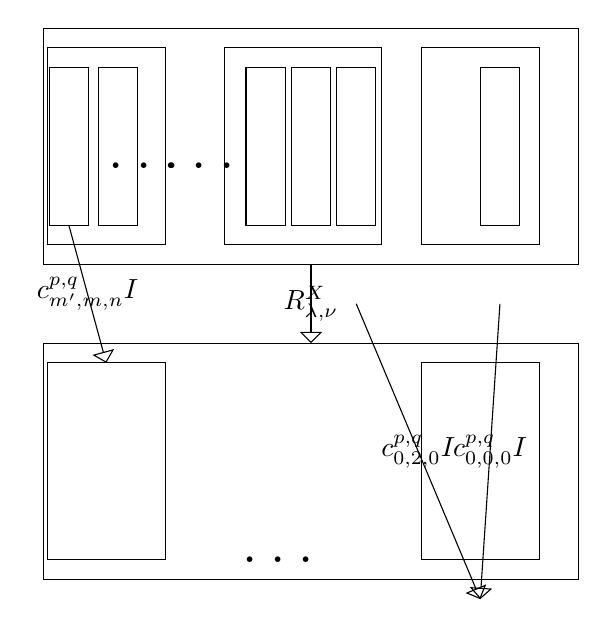
\begin{tikzpicture}[rotate=-90]
	\draw[color=black] (-9.0,0.75) rectangle (-6.0,-6.05);%upper
\draw[color=black] (-8.75,0.25) rectangle (-6.25,-1.25);%right in upper
\draw[color=black] (-8.5,0.0) rectangle (-6.5,-0.5);%in ``right in upper''
\draw[color=black] (-8.75,-1.75) rectangle (-6.25,-3.75);%middle in upper
\draw[color=black] (-8.5,-1.825) rectangle (-6.5,-2.325);%right in ``middle in upper''
\draw[color=black] (-8.5,-2.4) rectangle (-6.5,-2.9);%middle in ``middle in upper''
\draw[color=black] (-8.5,-2.975) rectangle (-6.5,-3.475);%left in ``middle in upper''
\draw[color=black] (-8.75,-4.5) rectangle (-6.25,-6.0);%left in upper
\draw[color=black] (-8.5,-4.85) rectangle (-6.5,-5.35);%right in ``left in upper''
\draw[color=black] (-8.5,-5.475) rectangle (-6.5,-5.975); %left in ``left in upper''

\draw[color=black] (-5.0,0.75) rectangle (-2.0,-6.05);%lower
\draw[color=black] (-4.75,0.25) rectangle (-2.25,-1.25);%right in lower
\draw[color=black] (-4.75,-4.5) rectangle (-2.25,-6.0);%left in lower

\node at (-7.25,-4.0) {\color{black}{\Huge \dots}};
\node at (-7.25,-4.7) {\color{black}{\Huge \dots}};
\node at (-2.25,-3.0) {\color{black}{\Huge \dots}};

%%\node at (-7.0,1.0) {\color{black}{$I(\lambda)$}};
%%\node at (-2.0,1.0) {\color{black}{$J(\nu)$}};

\draw[-open triangle 90] (-6.0,-2.65) to node {$R_{\lambda,\nu}^X$} (-5.0,-2.65);
\draw[-open triangle 90] (-5.5,-0.25) to node {$c^{p,q}_{0,0,0}I$} (-1.75,-0.5);
\draw[-open triangle 90] (-5.5,-2.075) to node {$c^{p,q}_{0,2,0}I$} (-1.75,-0.5);
\draw[-open triangle 90] (-6.5,-5.725) to node {$c^{p,q}_{m',m,n}I$} (-4.75,-5.25);

	\end{tikzpicture}
\end{center}
\end{frame}
\begin{frame}{アイディア}
	\begin{itemize}
		\item \ldots
		\item $\implies(K,K')$固有値がゼロになるかどうかを判定したい;
		\item<2-> $\mysbo$の積分核が別の手法で決定されたとする;
		\item<3-> $\implies(K,K')$固有値を積分の形で表示できる;
		\item<4-> $\implies$ 命題\ref{prop:int-st-gg}はガンマ関数の積公式として与えられるので
			ゼロかどうかが完全に決定できる.
	\end{itemize}
\end{frame}
\appendix
\begin{frame}[allowframebreaks]{References}
\end{frame}
%%\addtocounter{framenumber}{-3}
%%\begin{frame}[noframenumbering]{Gegenbauer多項式のロドリゲスの公式}
%%			\begin{equation*}
%%				(1-x^2)^{\alpha-\frac{1}{2}}C_n^\alpha(x)=a(\alpha,n)
%%				\frac{d^n}{dx^n} (1-x^2)^{n+\alpha-\frac{1}{2}},
%%			\end{equation*}
%%			\begin{equation*}
%%				a(\alpha,n)=\frac{(-1)^n}{2^nn!}\frac{\Gamma\left( \alpha+\frac{1}{2} \right)\Gamma\left( n+2\alpha \right)}{\Gamma(2\alpha)\Gamma\left(\alpha+n+\frac{1}{2}  \right)}
%%			\end{equation*}
%%\end{frame}
%%\begin{frame}[noframenumbering]{ンパクト群 O(n) の分規則 ルール}
%%	\begin{equation*}
%%		\mathcal{H}^L(\mathbb{S}^n)=\bigoplus_{N=0}^L \mathcal{H}^N(\mathbb{S}^{n-1}),
%%	\end{equation*}
%%	\begin{equation*}
%%		I_{N\to L}:\mathcal{H}^N(\mathbb{S}^{n-1})\to \mathcal{H}^L(\mathbb{S}^n),
%%	\end{equation*}
%%	\begin{equation*}
%%		\left(I_{N\to L}\varphi  \right)(\eta_0,\eta)=\myabs{\eta}^N\varphi\left( \frac{\eta}{\myabs{\eta}} \right)\tilde{\tilde{C}}^{\frac{n-1}{2}+N}_{L-N}(\eta_0).
%%	\end{equation*}
%%\end{frame}
%%\begin{frame}[noframenumbering]{命題\ref{prop:exp-stz-gg}$\implies$命題\ref{prop:exp-st-gg}}
%%\begin{equation*}
%%		{}_2F_1\left( \begin{array}[]{c}
%%			a,b\\c
%%		\end{array};1\right)=\frac{\Gamma(c-a-b)\Gamma(c)}{\Gamma(c-a)\Gamma(c-b)},\quad \Re(c-a-b)>0
%%	\end{equation*}
%%\end{frame}
%%\begin{frame}[noframenumbering]{超幾何関数に関数る等式}
%%	\[F\left(\begin{array}[]{c}
%%		a,1-a\\b
%%	\end{array}\tfrac{1}{2}\right)=\frac{2^{1-b}\sqrt{\pi}\Gamma\left(b\right)%
%%}{\Gamma\left(\tfrac{1}{2}a+\tfrac{1}{2}b\right)\Gamma\left(\tfrac{1}{2}b-%
%%\tfrac{1}{2}a+\tfrac{1}{2}\right)}.\]
%%\end{frame}
